\documentclass[a4paper 12pt]{article}
\usepackage[margin=1in]{geometry}
\usepackage{natbib}
\usepackage{epsfig}
\usepackage{amsmath}
\usepackage{amsfonts}
\usepackage{float}
\usepackage{rotating} 
\usepackage{caption}
\usepackage{subfig}
\usepackage{booktabs}
\usepackage{adjustbox}
\usepackage[table]{xcolor}
\usepackage{tabularx}
\usepackage{caption}
\usepackage{enumerate}
\usepackage{enumitem}
\captionsetup{font=footnotesize}
\newcommand{\ra}[1]{\renewcommand{\arraystretch}{#1}}
\textheight 9.0 in
\textwidth 6.5 in
%\topmargin -0.3 in
\oddsidemargin 0.0in
\renewcommand{\topfraction}{1}
\renewcommand{\bottomfraction}{1}
\renewcommand{\textfraction}{0}
\renewcommand{\floatpagefraction}{0.90}
\definecolor{TableEven}{rgb}{0.8000,0.9216,0.9490}
\usepackage{makecell}
%\usepackage{fourier} 
\numberwithin{equation}{section}
\usepackage{array}
\usepackage{titlesec}
\usepackage{sectsty}
\sectionfont{\centering}
\setcounter{secnumdepth}{4}
\usepackage{natbib}
\usepackage{siunitx}
\usepackage[toc,page]{appendix}
\usepackage{sectsty}
\usepackage{scalerel,stackengine}
\stackMath
\usepackage{graphicx}
\usepackage{amssymb}
\usepackage{xcolor}
\usepackage{hyperref}
\usepackage[normalem]{ulem} 

%\titleformat{\subsection}    
%       {\normalfont\fontfamily{phv}\fontsize{12}{17}\bfseries\itshape}{\thesubsection}{1em}{}
\subsectionfont{\normalfont\bfseries\itshape}
\subsubsectionfont{\normalfont\itshape}
%\usepackage[colorlinks,citecolor=DeepPink4,linkcolor=DarkRed, urlcolor=DarkBlue]{hyperref}
%\usepackage[svgnames]{xcolor} 
%
%\usepackage[colorlinks]{hyperref}
%\hypersetup{citecolor=DeepPink4}
%\hypersetup{linkcolor=DarkRed}
%\hypersetup{urlcolor=DarkBlue}
%\usepackage{cleveref}

%hyperlink for website will need a better option. highlights all equations etc
 \usepackage{hyperref}


\renewcommand{\baselinestretch} {2.0}
\makeatletter
\setcounter{page}{1}
\def\doublespace{\def\baselinestretch{1}\@normalsize}
\def\enddoublespace{}
\title{\bf 
}   
% \footnotemark}
\author{}
\date{}
\@addtoreset{equation}{section}
\renewcommand{\sp}{\vspace{0.2 in}}
\renewcommand{\theequation} {\arabic{section}.\arabic{equation}}
%\renewcommand{\thefigure}{\arabic{section}.\arabic{figure}}
\renewcommand{\thefootnote}{\fnsymbol{footnote}}
\newtheorem{theorem}{Theorem}
\newtheorem{lemma}{Lemma}[section]
\newtheorem{remark}{Remark}[section]
\newtheorem{corollary}{Corollary}[section]
\newtheorem{exam}{Example}[section]
\newtheorem{proposition}{Proposition}[section]

\newcommand{\Bigskip}{\vspace{0.3 in}}

\usepackage{xspace}
\newcommand{\m}{\textnormal{\sffamily m}\xspace}
\newcommand{\cm}{\textnormal{\sffamily cm}\xspace}
\newcommand{\g}{\textnormal{\sffamily g}\xspace}
\newcommand{\kg}{\textnormal{\sffamily kg}\xspace}
\newcommand{\SE}{\textnormal{\sffamily SE}\xspace}
\newcommand{\RSE}{\textnormal{\sffamily RSE}\xspace}
\newcommand{\LB}{\textnormal{\sffamily LB}\xspace}
\newcommand{\UB}{\textnormal{\sffamily UB}\xspace}


\newcommand{\mysquare}[1][black]{\small\textcolor{#1}{\ensuremath\blacksquare}}
\newcommand{\mycirc}[1][black]{\Large\textcolor{#1}{\ensuremath\bullet}}
\newcommand{\mylozenge}[1][black]{\small\textcolor{#1}{\ensuremath\blacklozenge}}
\newcommand{\mytriangle}[1][black]{\small\textcolor{#1}{\ensuremath\blacktriangle}}
\newcommand{\mydtriangle}[1][black]{\small\textcolor{#1}{\ensuremath\blacktriangledown}}
\newcommand{\mystar}[1][black]{\Large\textcolor{#1}{\ensuremath\star}} %% or \bigstar
%%%Syntax


% command for commenting
\usepackage{color}
\usepackage{ulem}
\newcommand{\ed}[1]{\textcolor{red}{#1}}
\newcommand{\nat}[1]{\textcolor{blue}{#1}}
\definecolor{darkgreen}{rgb}{0.09, 0.45, 0.27}
\newcommand{\olav}[1]{\textcolor{darkgreen}{#1}}

\newcommand{\natty}[1]{\textcolor{magenta}{#1}}

\makeatletter
\let\latex@xfloat=\@xfloat
\def\@xfloat #1[#2]{%
  \latex@xfloat #1[#2]%
  \def\baselinestretch{1}
  \@normalsize\normalsize
  \normalsize
}
\makeatother


\makeatletter
% \cvhrulefill{<color>}{<thickness>}
\newcommand*\cvhrulefill[2]{%
   \leavevmode\color{#1}\leaders\hrule\@height#2\hfill \kern\z@\normalcolor}
% \crule{<color>}{<width>}{<thickness>}
\newcommand*\crule[3]{%
   \color{#1}\rule{#2}{#3}\normalcolor}
\makeatother


\newcommand\longitude[1]{\directlua{ longitude ( \luastring{#1} ) }}


%\usepackage{lineno}
%\linenumbers

 
\begin{document}

%\title{An analysis of the North Sea International Bottom Trawl Survey Data}

\title{Evaluation of sampling strategies for age determination of Cod (\textit{Gadus morhua}) sampled at the  North Sea International Bottom Trawl Survey }
\maketitle


\begin{abstract}

The North Sea Cod stock assessment is based on indices of abundance-at-age from fishery-independent bottom trawl surveys. The age structure of the catch is estimated by sampling fish for otoliths collection in a length-stratified manner from trawl hauls. Since age determination of fish is costly and time-consuming, only a fraction of fish is sampled for age from a larger sample of the length distribution, and an age-length key (ALK) is then used to obtain the age distribution. Here, we evaluate ALK estimators for calculating indices of abundance-at-age, with and without the assumption of constant age length structures over relatively large areas. We also quantify the uncertainty of indices of  abundance and examine the effect of reducing the number of fish sampled for age determination on precision. For various subsampling strategies of otoliths collection, we show that  one fish per 5cm length group width per trawl haul is sufficient, and the total number of fish subsampled for age from trawl surveys could be reduced by at least half ($50\%$) without loss in precision.

\end{abstract}

% \citep{ehrhardt1997role}
\section{Introduction}
Fish stock assessments are used by fishery managers for making management decisions regarding catch quotas. These assessments provide fundamental information about the status of the stock, for instance, whether the stock is increasing and support for increased levels of harvest should be given, or whether the stock is decreasing and stricter control on harvest should be implemented. Associated with the parameters used in fish stock assessment are their uncertainties, which should not be ignored when formulating management policies \citep{ludwig1981measurement, berg2014evaluation}. These uncertainties can arise from many sources including natural variability, estimation procedures and statistical fitting. The North Sea International Bottom Trawl Survey (IBTS) data, coordinated by the International Council for the Exploration of the Sea (ICES), provides information on seasonal distribution of stocks and estimates of abundance indices and catch in numbers of fish per age-class without an assessment of the accuracy of these estimates. As stated by \citet{ludwig1981measurement} it is relevant for managers to take into account the uncertainty related to stock size when making management polices. The indices of abundance-at-age from IBTS  are based on data obtained from a stratified semi-random sampling approach of trawl stations,  and  it is essential to account for the sampling approach so as to produce reliable variance estimates \citep{lehtonen2004practical}. If the sampling approach is ignored, the effect on the variance  of the parameters could be substantial.  In particular, the variance could be greatly inflated (or deflated)  due to the clustering effect, which involves intra-cluster correlation of the variables \citep{aanes2015efficient, lehtonen2004practical}. 

There are two separate stages for generating indices of abundance-at-age from the North Sea International Bottom Trawl Survey (IBTS) data.  The first consist of calculating indices per \textit{length} class, which are obtained by trawling in a stratified manner, sorting the catch by taxa and taking biological measurement of the sorted catch. Then that knowledge is transformed to indices with respect to age. The latter part is achieved with an age-length key (ALK), which is constructed by subsampling otoliths from fish for age determination in a length-stratified manner from each haul and/or sub-area. To our best knowledge, there has been no research on how much the uncertainty of the abundance indices is related to these two distinct parts.

 Otolith sampling at the North Sea International Bottom Trawl Survey for age determination is quite extensive for both demersal and pelagic species. For  Cod (\textit{Gadus morhua}) in particular, otoliths from a subsample of one fish per 1cm length group width are collected from a larger length sample of approximately 100 Cod per haul. Since these fish are caught in clusters, their ages are more likely to be similar than those in the entire population, so there is positive intracluster correlation, and, therefore, less information on the age distribution is gained from taking (large) subsamples of otoliths from these clusters \citep{pennington1994assessing,aanes2015efficient}. The typical strategy for age sampling from 1991 to 2017 was quota sampling. For Cod, eight (8) age samples per 1cm length group width in a round fish area were taken. This sampling strategy is not representative of the population as quotas could be reached before the entire survey area is covered. 

In this research, we determine the precision of estimates of relative abundance-at-age of the North Sea International Bottom Trawl Cod (\textit{Gadus morhua}) by applying two different age-length key (ALK) estimators \citep{fridriksson1934calculation}. We also focus on the spatial distribution of the ALK. Relative abundance indices of the North Sea IBTS are estimated using an age-length key (ALK) that assumes age-length structures are constant over relatively large areas. We propose a design-based ALK, referred to as haul based ALK that accounts for spatial variation of the fish parameters. Spatial structures in the ALK have also been investigated in \citet{berg2012spatial} and  \citet{hirst2012bayesian}. In addition, because age determination of fish is time consuming, we examine whether the number of fish aged from each haul could be reduced without significantly reducing the
precision of the estimates. We achieve the reduction of the number of fish aged by mimicking a sampling procedure with less effort.

An  overview of the  North Sea International Bottom Trawl Survey is given in Section \ref{overview}. The current estimators for ALK and catch per unit effort (CPUE) used by ICES in their database for trawl surveys (DATRAS) and our proposed ALK estimator are given in Section \ref{sec:methods}. We apply these ALK methods to a case study in Section  \ref{sec:data}, and a discussion is given in Section \ref{sec:discussion}. The R-code for reproducing the results can be fund at github (\href{https://github.com/natoyaj/TestPackage.git}{https://github.com/natoyaj/TestPackage.git}). % \natty{(rename package and place on S2D or imr github address)}.
 

\subsection{Overview of the North Sea International Bottom Trawl Survey}
\label{overview}
\indent The North Sea International Bottom Trawl Survey was formed in 1991, to combine the International Young Herring Survey (IYHS) and eight national surveys in the North Sea, Skagerrak and Kattegat areas. These surveys began in the 1960's, and the 1970's and 1980's, respectively. The IYHS was developed with the aim of obtaining annual recruitment indices for the combined North Sea herring (\textit{Clupea harengus}) stock \citep{ICES2012}, but yielded valuable information on other fish species such as Cod (\textit{Gadus morhua}) and haddock (\textit{Melanogrammus aeglefinus}).

\indent The North Sea IBTS began with quarterly surveys providing information on seasonal distribution of stocks, which allows changes in fish stock to be monitored and abundance of all fish species to be determined. These quarterly surveys, however became difficult to sustain as countries experienced budget cuts making it impossible to maintain high levels of research vessel effort. As such, in 1997 countries carried out a survey only twice a year; a first quarter survey (January-February) and a third quarter survey (July-September). The target species of IBTS fished from 1991-2018 includes standard pelagic species: Herring (\textit{Clupea harengus}), Sprat (\textit{Sprattus sprattus}) and Mackerel (\textit{Scomber scombrus}); and standard roundfish species: Cod (\textit{Gadus morhua}), Haddock (\textit{Melanogrammus aeglefinus}), Saithe (\textit{Pollachius virens}),  Norway Pout (\textit{Trisopterus esmarkii})  and Whiting (\textit{Merlangius merlangus}). There are also several by-catch species \citep{ICES2006Report}

Research vessels from seven nations in the first quarter (Q1) and six nations in the third quarter (Q3) are used for conducting surveys on all finfish species in the North Sea during January-February and July-August, respectively, between 1997-2018. Table \ref{countries} in Supplementary Materials \ref{secAp:areasfishedappendix} gives details of the research vessels. The sampling frame is defined by the ICES index or roundfish areas (RFA) as shown in Figure \ref{icesroufismap} numbered 1 to 10. These  roundfish areas were substratified into small strata defined by non-overlapping statistical rectangles of roughly $30 \times 30$ nautical miles ($1^{o} \  \mathrm{Longitude} \ \times  \  0.5^{o} \ \mathrm{Latitude}$), and were convenient to use for IBTS as they were already being used for fisheries management purposes. Most statistical rectangles contain a number of possible trawl hauls or tows that are deemed free of obstructions. These tows, which are referred to as   "safe tows", are taken from national databases of participating countries, DATRAS \citep{datras} or commercial fishing data. While nations are free to choose any position within a statistical rectangle to sample, tows are generally selected based on a semi-random approach from these safe tow locations. However, some nations such as Sweden and England use fixed tows, and in some cases Sweden utilizes a depth-stratified semi-random sampling design of tows \citep{ICES2018}. Sampling may be further stratified, in some statistical rectangles, due to significant changes in seabed depth which may, in turn, cause variations in the fish population. In particular, the North Sea IBTS herring, Saithe and sprat data are weighted by depth strata in the statistical rectangle \citep{ICES2013}. It is a requirement that tow locations be at least 10 nautical miles within and between statistical rectangles \citep{ICES2018}. Also, a target coverage of two tows is required per statistical rectangle\citep{ICES2015}, but in some statistical rectangles in the Eastern English Channel, Southern North Sea and Central North Sea intensified sampling is carried out.

The recommended standard trawling gear of the North Sea IBTS is the mulitpurpose chalut {\`a} Grande Ouverture Verticale (GOV) trawl \citep{ICES2012}, which has been used on all participating vessels since 1992, while different pelagic and bottom trawls suitable for fishing finfish species were used before 1992. Standardized trawling protocols were adopted with a towing speed of 4 knots but depending on vessel performance, tide and weather conditions the average towing speed can be at minimum 3.5 and maximum 4.5 knots. A tow duration of 30 minutes was adopted by all nations in 1999, but in the third quarter (Q3) of 2015, an experiment on tow duration was conducted in the North Sea to investigate the effect on the composition of catches. This experiment continued into the first quarter of 2016 with one participating nation \citep{ICES2016c}.  In rectangles with two hauls allocated, tow duration of one of the hauls was reduced to 15 minutes while 30 minutes tow duration was maintained for the other one. Four nations  participated in this exercise, and therefore, no mixed tow durations were planned for the Skagerrak, which is almost exclusively covered by Sweden (see Table \ref{countries} in Supplementary Materials \ref{secAp:areasfishedappendix} for all nations participating in the North Sea IBTS). The introduction of 15 minutes tows allowed the extension of the survey area and resulted in a much more balanced coverage of the North Sea than in previous years. Also, there was no indication that the shorter tows were less efficient than the standard 30 minutes tows for catching larger and/or older fish in 2015 Q3. But in the first quarter of 2016 the shorter tows caught fewer species, the catch rates in numbers and weight were larger, and the individuals caught were smaller  \citep[see][]{ICES2016c}. 

Trawling is done during the daylight hours, which are considered 15 minutes before sunrise to 15 minutes  after sunset \citep{ICES2012}. After each trawl the total catch of the different species is weighed on board and biological parameters such as length for all fish species caught are collected. Where the numbers of individuals are too large for all of them  to be measured to obtain the length distribution, a representative subsample of 100 fish is selected. A pair of otoliths are collected on board from a small fraction of all the target species from all RFAs (Figure \ref{icesroufismap}) to retrieve age reading. Table \ref{tab:otolithsTable} in Supplementary Materials \ref{secAp:otolithappendix} gives the minimum sampling levels of otoliths for the target species.
 %Denmark, Germany, Norway, and Scotland
 %This is a direct contradiction to what was found in the 2015 Q3 survey. no indication was found that the shorter tow were less efficientthan the standard 30 min tows for catching larger and/or older fish. Species richness on the other hand appeared to be slightly lower in the short than in the long tows due to the smaller fished area. They indicated neither a significant effect of tow duration on the abundance indices of NS-IBTS target species, nor on the total number of species recorded
 
%\clearpage
\begin{figure*}[h!]
\centering
\begin{tabular}{@{}ccc@{}}
\subfloat[]{\includegraphics[width=0.95\textwidth]{figures/Maps/surveyarea}} & 
\end{tabular}
\caption[]{Standard roundfish areas (RFAs) used for roundfish since 1980 and for all standard species since 1991 (left panel). RFA 10 was added in 2009. The number 1, for example, indicates ICES RFA 1. The small grey rectangles in the left panel indicates the statistical rectangles of approximately $30 \times 30$ nautical miles (these vary from ~28 nm wide in the north, to ~40 nm wide in the south of North sea) ($1^{o} \  \mathrm{Longitude} \ \times  \  0.5^{o} \ \mathrm{Latitude}$). The map in the right panel shows the Norwegian trench and shelf edge (depths 1000-1500).}
\label{icesroufismap}
\end{figure*} 

\section{\large METHODS}
\label{sec:methods}
This section gives the estimators of abundance indices. The estimators are haul-duration based and utilizes an ALK approach. We consider the ALK approach used in DATRAS and we propose two ALK estimators. The ALK used in DATRAS assumes constant  age-length structures over large areas, see roundfish areas in Figure \ref{icesroufismap}.  As differences in age-length structures may exist over large areas, these differences do have the potential to result in a biased ALK \citep{gerritsen2006simple,kimura1977statistical}. To account for the spatial distribution we propose a design-based ALK that is haul dependent (Section \ref{sec:haulestimator}).

\subsection{Catch per unit effort}
\label{sec:cpueestimators}
In this research, the catch per unit effort (CPUE) is defined as the number of fish of a certain species and age or length which are caught per hour trawl. In this section we define the CPUE mathematically, which explains how the index is calculated. For a given species of interest, let $n_{h,l}$ be the number of fish with length $l$ caught by trawl haul $h$. The CPUE for a given length $l$ by trawl haul $h$ is defined as 
\begin{equation}\label{eq:cpueHaul}
\mathrm{CPUE}_{h,l} =\frac{n_{h,l}}{d_h},
\end{equation}
were $d_h$ is the duration of the trawl in hours. The CPUE per age class is further defined as
\begin{equation}\label{eq:cpueALK}
\mathrm{CPUE}_{h,a} =\sum_{l \in {\bf L}}\mathrm{CPUE}_{h, l} \times ALK_{a,l,h},
\end{equation}
where ${\bf L}$ is the set of all length classes and $ALK_{a,l,h}$ represents the estimated proportion of fish with age $a$ in $l$th length class in haul $h$. The mean CPUE per age in a statistical rectangle $s$ is further defined as
\begin{equation}\label{eq:cpueRec}
\mathrm{mCPUE}_{s,a} =\frac{\sum_{h \in H_{s}} \mathrm{CPUE}_{h,a}}{|H_{s}|}.
\end{equation}
Here, $H_{s}$ represents the set of trawl hauls taken in statistical rectangle $s$, and $|H_{s}|$ is the number of hauls taken in the rectangle. The mCPUE in $p$th RFA is further defined as
\begin{equation}\label{eq:cpueRFA}
\mathrm{mCPUE}_{p,a} = \frac{ \sum_{s \in S_{p}} \mathrm{mCPUE}_{s,a}}{|S_{p}|} \omega_s,
\end{equation}
where $S_{p}$ is the set of all statistical rectangles in RFA $p$, $|S_{p}|$ is the number of statistical rectangles in RFA $p$, and $\omega_s$ is a weight factor for each statistical rectangle \citep{ICES2013}. For species such as Saithe, herring, and sprat the indices at age are calculated using the mean over rectangles, weighted for the percentage of area with water depths between 10m-200m, and for RFAs 8 and 9 water depths between 10m-250m \citep{ICES2013}.

 The mean catch per unit at age in the whole study area is defined as
\begin{equation}
\text{mCPUE}_a= \frac{\sum_{p\in {\bf P}} A_{p}  \mathrm{mCPUE}_{p,a}}{A_{\text{total}}}.
\label{eq:abundanceestimatornorthsea}
\end{equation}
We refer to (\ref{eq:abundanceestimatornorthsea}) as the index of abundance-at-age, where ${\bf P}$ is the set of RFAs, $A_p$ is the area of RFA $p$, and $A_{\text{total}} = \sum_{p\in {\bf P}} A_{p}$. This index takes into account, the entire survey area of the North Sea IBTS (Figure \ref{icesroufismap}). 
%mCPUE_{N,a} 
\subsection{ALK estimators}
\label{sec:alkmethods}
The estimator of the CPUE of age includes an ALK, see (\ref{eq:cpueALK}), which we describe in this section. Two ALKs are included in this research. The first is an ALK estimator currently used by ICES for estimating IBTS abundance indices of North Sea Cod \cite{ICES2013}, but these estimates are not used in assessment models. We refer to this ALK estimator as the area based ALK. The second is an alternative ALK estimator, which we propose to account for spatial variation in age-length compositions. We refer to this ALK as a haul based ALK.

\subsubsection{Area based ALK}
\label{sec:datrasalkestimator}
We denote the area based ALK used in DATRAS as $ALK^{\text{A}}_{a,l,h}$. The area based ALK is defined as constant within each RFA, and is calculated for each RFA by aggregating the age observation from each RFA. $ALK^{\text{A}}_{a,l,h}$ used in equation (\ref{eq:cpueALK}) is defined as the proportion of observed fish with age $a$ in length class $l$ in the corresponding RFA. If there are no observed fish in length class $l$ in the RFA, ages from length classes close to $l$ is used. This is referred to as borrowing of ALKs for imputation of missing values. Note that borrowing of ALKs for imputation is a common practice in analysis of both fishery-independent and fishery-dependent monitoring data \citep[see for example,][]{aanes2015efficient,catchpole2017challenges}. The details of the procedure for borrowing age data from neighbouring length classes are as follow: If there does not exist an age reading of a fish of length $l$ in an RFA,  \citet{ICES2013} propose that the following procedure  for the area based ALK be adopted:
\begin{enumerate}
\item If $l$ is between the minumum length and maximum length, the age is set to be equal the ALK to the closest length group with observed ages in the RFA. In cases where there are two equally close length groups with observed ages, the average of those two ALKs is used. 
\item If $l$ is smaller then the smallest measured fish in the RFA, the age is set to the minimum age.
\item If $l$ is larger or equal the maximum length, the age is set to the maximum age.
\end{enumerate}
The underlying assumption of this ALK  is that age-length compositions are homogeneous within the RFAs. This is a rather strong assumption, and any violation would have some impact on the estimates of abundance indices and their variability. For instance,  \citet{aanes2015efficient} illustrated that a violation of the assumption of constant ALK leads to biased estimates of CPUEs. 

\subsubsection{Haul based ALK}
\label{sec:haulestimator}
We denote the haul dependent ALK  by  $ALK^{H}$. The $ALK^{H}_{a,l,h}$  used in equation (\ref{eq:cpueALK}) is defined as the average proportion of observed fish with age $a$ in  length class $l$ in haul $h$. If there are no observed ages of fish in a length class $l$ in the haul, we propose the following for filling missing age-length keys in the  haul based procedure, in sequential order:
\begin{enumerate}
\item If there exist an age reading of that length group less than or equal to 60 nautical miles in the same RFA, the ALK from the closest haul with such an age reading is used.
\item If there exist a fish with length in the interval $l\pm 1cm$ with age information in the same haul, that observed age is used.  
\item If steps 1 an 2 do not produce an ALK for $l$, there exist little information close in space and length, and the area based ALK is used. %(\ed{did we actually do this step? I thought Sondre and Jon Helge said to stop if this happens. Alternatives are 1) model base approach or removing areas from the study where ages are lacking. Because if we do this, we are implementing exactly what DATRAS did}). \olav{We currently do this step. This step is done for relatively few fish. I suggest we argue that this step has minor effect on the estimate by illustrating the portion of fish which are mapped from length to age by this step. We can delete those areas, but then I think there is a loot of pitfalls to get into. I suspect these hauls are in areas with little catch of the species of interest, and care must be taken if deleting those areas/hauls without getting biased estimates.}
\end{enumerate}

\subsection{Uncertainty estimation}
\label{sec:uncertaintyestimation}
In this section we describe how the uncertainty of the CPUE estimates are calculated. We use nonparametric bootstrapping to quantify the uncertainty of the CPUEs. Nonparametric resampling allows us to estimate the sampling distribution of the CPUE empirically without making assumptions concerning the data. A bootstrap procedure for estimating the uncertainty of CPUEs in the North Sea is suggested in \citet{ICES2006Report}. We refer to this procedure as ICES-IBTS bootstrap procedure. In this research we implement the ICES-IBTS bootstrap procedure along with a modification, which we refer to as modified ICES-IBTS bootstrap procedure. We also implement a bootstrap procedure that accounts for stratification in the multistage sampling design. This procedure is referred to as the stratified bootstrap procedure. These procedures are described in detail in Section \ref{sec:datrasstratifiedbootstrap}. Approximate $95\%$ confidence intervals are obtained using the bias-corrected percentile method  \citep{gavaris2002statistical, magnusson2013measuring}. The bias-corrected method adjusts for the bias and skew of the sampling distribution of the data, and has shown to lead to more accurate confidence intervals   \citep{efron2003second,restrepo2000different}. 

\subsubsection{Bootstrap procedures}
\label{sec:datrasstratifiedbootstrap}
This section describes the bootstrap procedures used in this research. The bootstrap procedures are constructed as follow:

%(\ed{Perhaps the order so be as follows: give the DATRAS bootstrap procedure, and its modification. Then give the bootstrap procedure we are suggesting to account for the stratification in the sampling design). This is way, it would be much clearer to the reader to identify the three procedures)}

\begin{enumerate}
\item For each statistical rectangle $s$, sample $|H_s|$ hauls and assign them to statistical rectangle $s$. We implement the following two procedure for this step. The procedure (a) is suggested by \citep{ICES2006Report}, and procedure (b) is our suggestion for the modified ICES-IBTS and the stratified  bootstrap procedures, which is intended to account for the sampling design: 
\begin{enumerate}
\item Sample $|H_s|$ hauls with replacement from the corresponding RFA.
\item sample $|H_s|$ hauls with replacement from the corresponding statistical rectangle. If there is only one haul within a statistical rectangle, sample either that haul or the closest haul.
\end{enumerate}
\item Sample age observations from the resampled hauls obtained in step 1. We implement the following two procedures for this step. Again, the procedure (a) is suggested by \citep{ICES2006Report}, and is implemented for ICES-IBTS bootstrap procedure and the modified ICES-IBTS bootstrap procedure. Procedure (b) is our suggestion for the stratified bootstrap procedure, which is intended to account for sampling design: 
\begin{enumerate}
\item For each \textit{RFA} and length group $l$, sample with replacement $n_{RFA,l,a}$ age observations stratified with respect to \textit{RFA} and length group. Here $n_{RFA,l,a}$ is the total number of age observations in length group $l$ in the corresponding RFA. If there is only one observed age from a given length group, i.e. $n_{RFA,l,a} = 1$, we sample either that age or an age in the closest length class with observed ages within the RFA.
\item For each haul and length group, sample without replacement  $n_{l,a,h}$ age observations stratified with respect to haul and length group using a pseudo-population bootstrap procedure \citep{mashreghi2016survey}. Here $n_{l,a,h}$ is the total number of age observations in length group $l$ in the corresponding haul. If there is only one observed age within a length group in a haul, that age is sampled. The pseudo bootstrap procedure is presented in Supplementary Materials \ref{secAp:pseudobootstrap}. 

\end{enumerate}
\item Calculate the relative abundance-at-age, $\text{mCPUE}_a$ in (\ref{eq:abundanceestimatornorthsea}), using the sampled data.
\item Repeat 1-3 B times, where B is the number of bootstrap replications.
\end{enumerate}

%We choose $n_{l,a,h}$ equal \textit{one} or \textit{two} when sampling the reduced effort
\subsection{Reducing the number of otoliths sampled for age determination}
\label{sec:reducingeffort}
We also investigate how relative abundance-at-age, $\text{mCPUE}_a$, and its uncertainty are affected if the  number of otoliths sampled for age determination is reduced. We sample realisations of data obtained with a sampling procedure with fewer age readings by choosing the number of age observations in length group $l$ in the corresponding haul,  $n_{l,a,h}$ (defined in step 2 (b) in Section \ref{sec:datrasstratifiedbootstrap}) to be equal to a pre-defined number. By doing that, the sampled data sets in the bootstrap procedure are possible realisations of data obtained by collecting a pre-defined number of otoliths for age determination. We investigate the effect on estimated relative abundance and its variability by considering two sampling procedures: firstly,  we sample \textit{one} fish for age determination from length group width 1\text{cm}, 2\text{cm}, 3\text{cm}, 4\text{cm} \text{ or }5\text{cm}; secondly, we set a length group width of 5\text{cm} and we sample \textit{one}, \textit{two}, \textit{three}, \textit{four} or \textit{five} fish for age determination. These procedures would capture the variability in age-length data, and allow sufficient sample sizes of otoliths required to give information on relative abundance-at-age in the North Sea to be determined. 

\subsection{Evaluating the effect of the number trawl hauls on relative abundance}
\label{sec:evaluatingtrawlhauls}
Several research studies have shown that the precision in estimates of age-compositions is primarily driven by the number of trawl hauls and not the number of fish measured for age \citep{aanes2015efficient, sondre2003estimating, stewart2014bootstrapping}. We therefore investigate the effect of reducing the number of fish sampled for age determination, and reducing (or increasing) the number of hauls on the expected relative standard error of abundance-at-age of the North Sea Cod. We use the sampling procedure described in Section \ref{sec:reducingeffort} to sample fish per length group width for age determination. The bootstrap procedure used to sample trawl hauls is described below. Let $N$ be the number of trawls to be sampled:
\begin{enumerate}
\item Sample $N$ hauls, stratified with respect to RFA, such that the proportion of hauls between RFAs is approximately the same as in the original survey design.
    % \begin{enumerate}
     % \item stratified with respect to RFA 
   %   \item from each RFA such that the proportion of hauls between RFAs is the same as the original survey design. We restrict the sampling experiment such that no fewer than two hauls in a RFA are sampled.
%      \end{enumerate} 
\item Sample age stratified with respect to length from the hauls sampled in step 1) above, using the pseudo-bootstrap procedure described in Section \ref{sec:datrasstratifiedbootstrap} and in Supplementary Materials \ref{secAp:pseudobootstrap}.
\item Calculate CPUE per age using the area based ALK.
\item Repeat 1-3 B times, where B is the number of bootstrap replicates.
\end{enumerate}

%Suggest we do not use a) and b) here. We can write:" Sample N hauls stratified with respect to RFA such that the proportion of hauls between RFAs is approximately the same as in the original survey design. "
%We do not sample stratified to statistical rectangle because there are to few observations in the statistical rectangles to achieve any large reduction.


\section{Case Studies}
\label{sec:data}
In this section we apply the methods described in Section \ref{sec:methods} to data for Cod from the International Bottom Trawl Survey for the years 2015-2018 in the first (Q1) and third quarters (Q3), which is obtained from the DATRAS database (\href{https://datras.ices.dk}{https://datras.ices.dk}). These years are chosen for two reasons. The first is that in year 2018 new sampling procedures proposed by ICES for the collection of otoliths for age determination were introduced in the surveys (see Table \ref{tab:otolithsTable} in Supplementary Materials \ref{secAp:otolithappendix} for sampling procedures). The second is that the years 2015-2018  provide extensive sample data with quarterly sampling effort varying between 345 and 387 trawl hauls.  For each of these hauls sampled in the years 2015-2018, concurrent length measurements and otoliths were obtained from a subsample of North Sea Cod. The number of otoliths collected for age determination in these years varies between 1456 and 2895. We also use both Q1 and Q3 data, which has different age spans, to evaluate the sampling strategy for both quarters. 
%The North Sea IBTS included age 0 in Q3 surveys and these data must be included when creating the age-length keys.

In the stock assessment of the North Sea Cod,  ICES considers age groups 0 to $6+$ from IBTS surveys data, where the last group is referred to as a ``plus group'', and which consists of fish of age 6 or older.  In this research, we consider age groups 1 to $6+$ in the first quarter and 0 to $6+$ in the third quarter. Table \ref{tab:realdata2017-2018Cod} in Supplementary Materials (\ref{secAp:data}) gives a brief summary of the data.

\subsection{Evaluation of ALK estimators}
\label{sec:EstimatesALK}
In this section we provide estimates of the mean catch per unit effort at age ($mCPUE_{a}$) or the relative abundance of the North Sea Cod  and their uncertainties from the two ALK estimators (\ref{sec:alkmethods}) and bootstrap procedures (\ref{sec:datrasstratifiedbootstrap}). Figure \ref{AreaHaulEstimatesAllYearsQ1} gives estimates for years 2015-2018 Q1 for 500 bootstrap samples. The area based ALK and haul based ALK gave similar point estimates of $mCPUE_{a}$, and similar performance is achieved between the two ALK estimators with respect to variability. This suggests that how we include the uncertainty in ALK the in the estimation process has minor importance, and that the uncertainty is likely to be caused by some other factor other than the uncertainty in the ALK. Estimates of mean catch per unit effort are dominated by  2-year-old fish in 2015 and by 1-year-old fish in 2017.

 With regard to the bootstrap procedures for variance estimation, ICES-IBTS procedure gave higher estimates of the variance compared with the modified ICES-IBTS and stratified procedures (Figure \ref{AreaHaulEstimatesAllYearsQ1}, right panel). Recall that  ICES-IBTS bootstrap  procedure ignores the fine scale stratification at the first stage (step 1. (a)  in Section \ref{sec:datrasstratifiedbootstrap}), and thus, overestimates the uncertainty. ICES-IBTS bootstrap procedure also ignores age-length data collected at the haul level, resulting in an underestimation in the uncertainty. So, there is bias in both direction. However, as illustrated in Figure  \ref{AreaHaulEstimatesAllYearsQ1}, the underestimation due to the ALK seems to be small. The modified ICES-IBTS and stratified bootstrap procedures sample hauls at the level of the statistical rectangle, and these procedures gave lower variance estimates presumably because too few hauls are available for resampling (maximum two hauls per statistical rectangle). \nat{Visual inspection of fish of a given length caught in hauls suggests that fish of similar sizes tend to aggregate together (see for example, Figure \ref{HaulsAndAgeCorrelation} (c)). Furthermore, fish caught at a trawl station are more likely to have similar age given length than those in the entire population,  so there is intra-cluster correlation, and even at low levels can greatly increase the variance of the estimated mean catch per unit effort at age \citep{pennington1994assessing}}. These results along with the RSEs (Figure \ref{AreaHaulEstimatesAllYearsQ1}, right panel), and  the distribution of North Sea Cod across hauls (Figure \ref{HaulsAndAgeCorrelation}) indicate that the variance is primarily driven by the hauls, hence, the higher variance from ICES-IBTS bootstrap procedure.
 
 %I don't understand how we can see this from figure 2. Can we see that from the figure?
 %But we argue above that it does not do so in our situation. If we include this scentene we should perhaps include that "but in our case study it seems to be have a minor effect on the variance".
 %But it is not much higher than for age 0. As i can see the RSE is larger for age 0 than for age 3 in that year and quarter.  I think it is good we include that the uncertainty seems to be driven largely from one haul with relatively high catch of age 3 and 4 cod.
Similar trends are observed in the third quarter, where juvenile North Sea Cod (2-year-old and the 0-group) dominates the estimates (Figure \ref{AreaHaulEstimatesAllYearsQ3} In Supplementary Materials \ref{secAp:estimatesFromALK}) . In 2018 Q3, the uncertainty in 3-year-old and 4-year-old fish is high compared to the younger age classes, except for age 0, and with expected relative standard error exceeding 25\%. This high variance is driven by a single haul (Figure \ref{HaulsAgeTotalAllYearsCod2018Q3} in Supplementary Materials \ref{secAp:estimatesFromALK}), which dominates the catch of 3 or 4 year-old fish.  \\

\clearpage

\begin{figure*}[h!]
\centering
\captionsetup{font=small, width = 15.5cm}{
\caption[]{Hauls containing age samples of North Sea Cod in 2015 Q1 and 2018 Q1 and the corresponding maps with the geographical location of hauls with these age samples in the North Sea. The coloured circles in graphs (b) and (d) are the hauls corresponding to the age of a fish in graphs (a) and (c), respectively. Fish of similar sizes tend to aggregate together, so the variability of catch at age given length within hauls is likely to be lower comapred with the variabililty across stations.} \label{HaulsAndAgeCorrelation}}
\begin{tabular}{@{}ccc@{}}
\subfloat[]{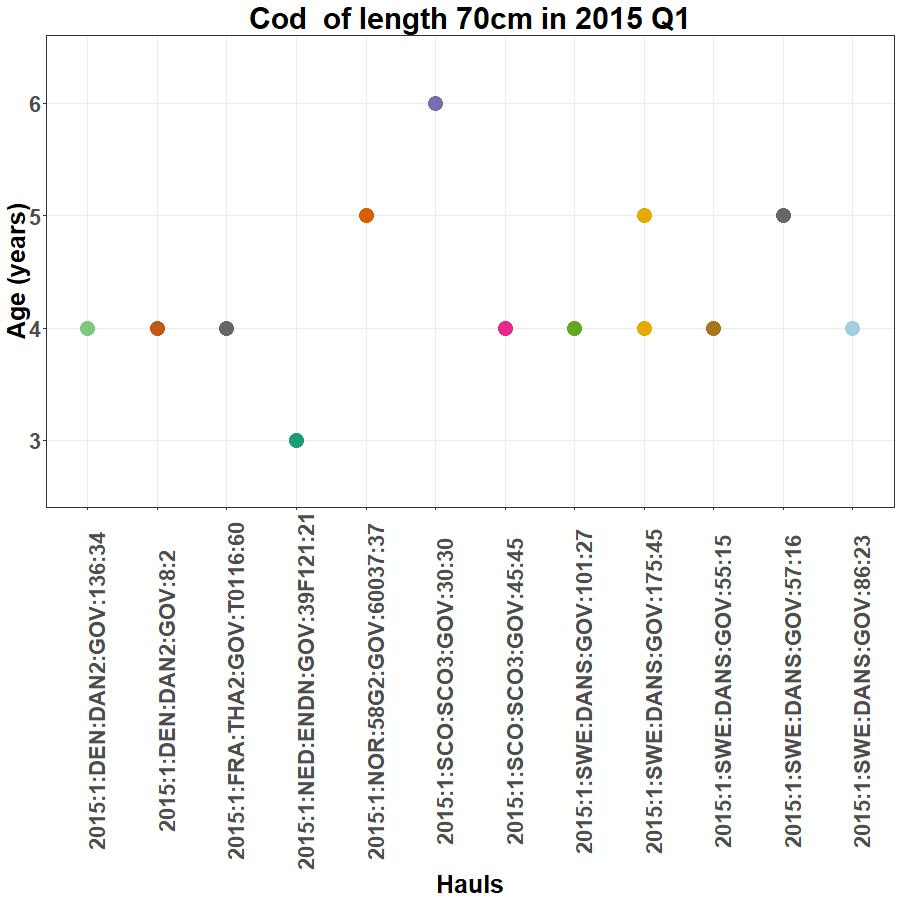
\includegraphics[width=0.38\textwidth]{figures/CorrelationofAgeInHauls/Length70cm2015Q1.jpeg}}
\qquad
\subfloat[]{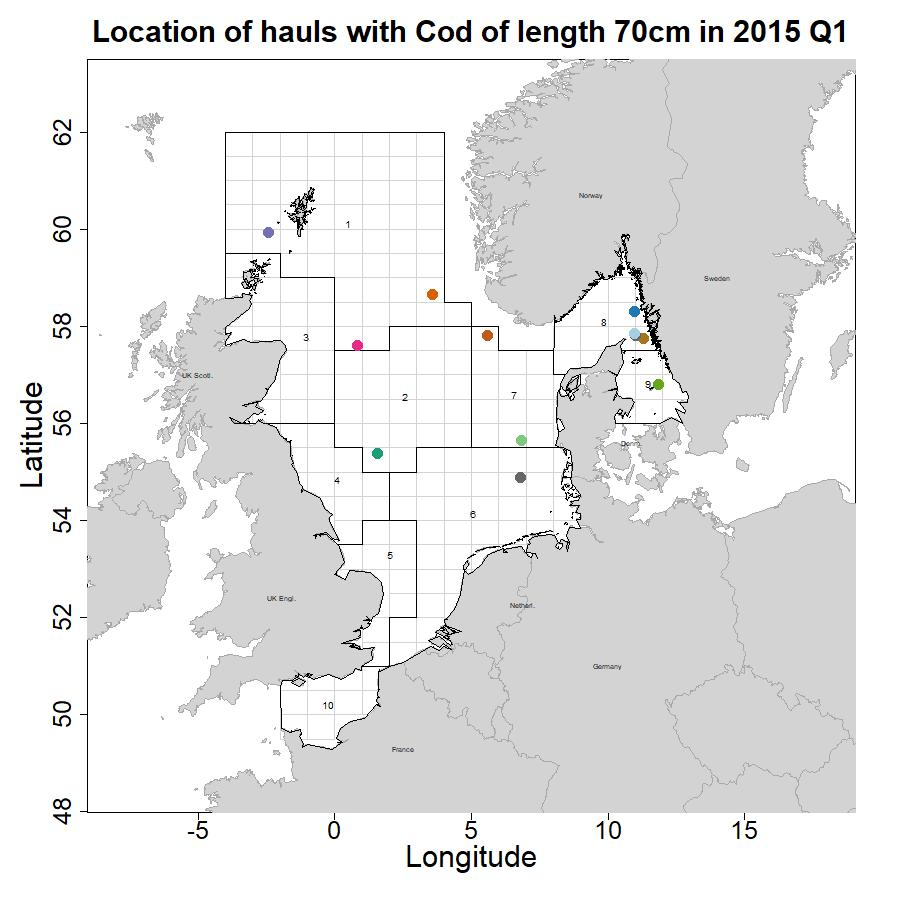
\includegraphics[width=0.38\textwidth]{figures/CorrelationofAgeInHauls/Map70cm2015Q1.jpeg}}  \\
\qquad
\subfloat[]{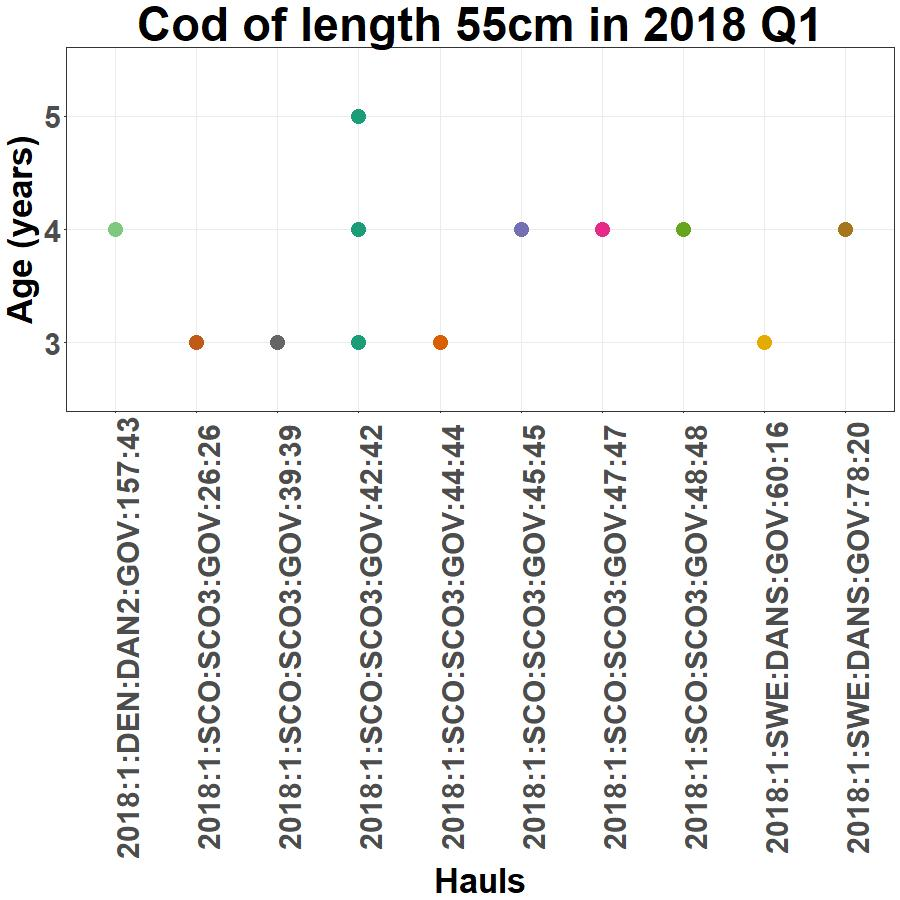
\includegraphics[width=0.38\textwidth]{figures/CorrelationofAgeInHauls/Length55cm2018Q1.jpeg}}
\qquad  
\subfloat[]{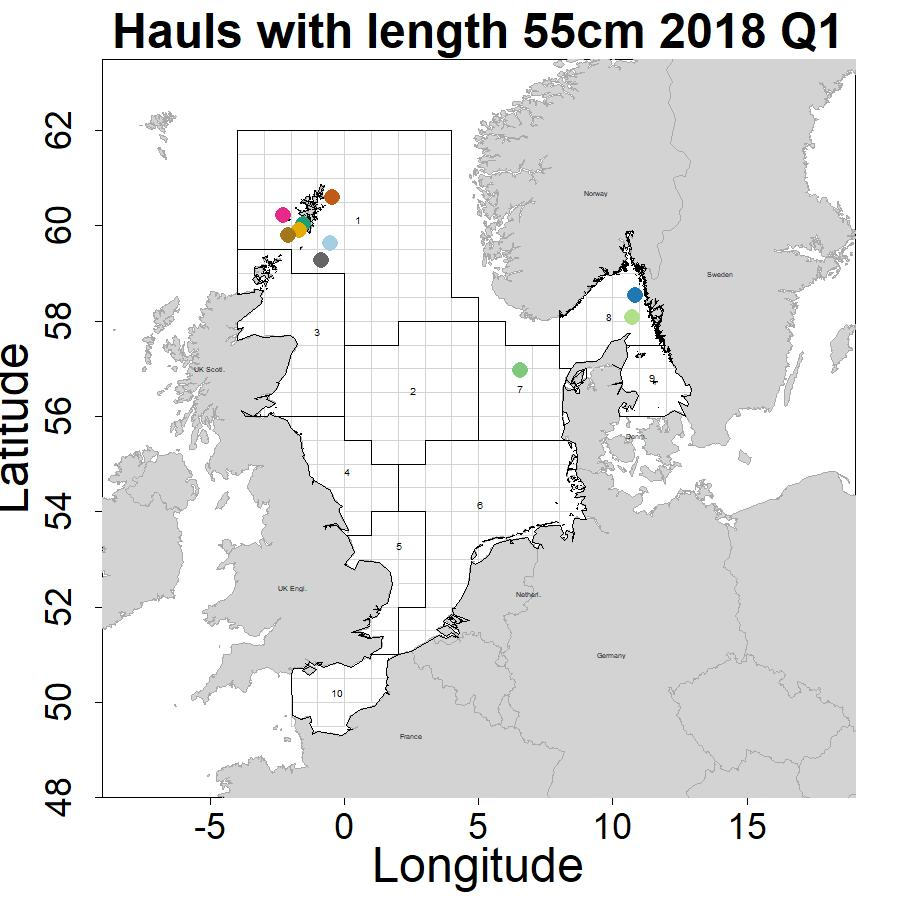
\includegraphics[width=0.38\textwidth]{figures/CorrelationofAgeInHauls/Map55cm2018Q1.jpeg}}  
\end{tabular}
\end{figure*} 


%Figure \ref{HaulsAndAgeCorrelation} gives the age and spatial distribution of North Sea Cod of lengths 55cm or 70cm in the first quarter (Q1) in years 2015 and 2018, respectively.\\
%The expected relative standard error from the ICES-IBTS bootstrap procedure, generally exceed those from the modified ICES-IBTS and stratified bootstrap procedures (Figure \ref{AreaHaulEstimatesAllYearsQ1}, right panel). ICES-IBTS bootstrap  procedure ignores the fine scale stratification at the first stage (step 1. (a)  in Section \ref{sec:datrasstratifiedbootstrap}), resulting in an overestimation of the uncertainty. ICES-IBTS bootstrap procedure also ignores age-length data collected at the haul level, resulting in an underestimation in the uncertainty, hence, there is bias in both direction. 


\clearpage
\begin{figure*}[h!]
\centering
\captionsetup{font=small, width = 14.5cm}{
\caption[]{Estimated mean catch per unit effort at age of North Sea Cod from the two ALK estimators based on data from the International Bottom Trawl Survey in 2015-2018 in the first quarter Q1 (left panel). The error bars are estimated 95\% confidence intervals using the bias corrected (see Methods) and 500 bootstrap samples. Expected relative standard error (RSE) for estimated abundance-at-age ($mCPUE_{a}$) are also given in the right panel. The ICES-IBTS bootstrap procedures are applied to the area based ALK and the stratified bootstrap procedure is applied to the haul based ALK.}\label{AreaHaulEstimatesAllYearsQ1}}
\begin{tabular}{@{}ccccc@{}}
\subfloat[]{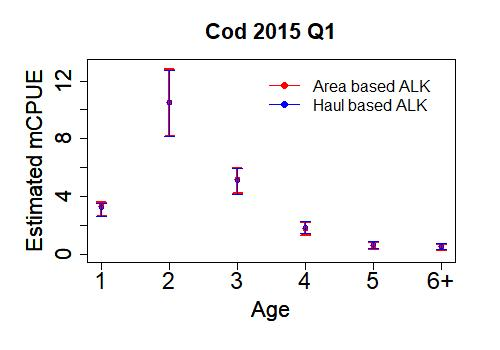
\includegraphics[width=0.33\textwidth]{figures/ALKplots/CodAreaHaulEstimates2015Q1.jpeg}} & 
\subfloat[]{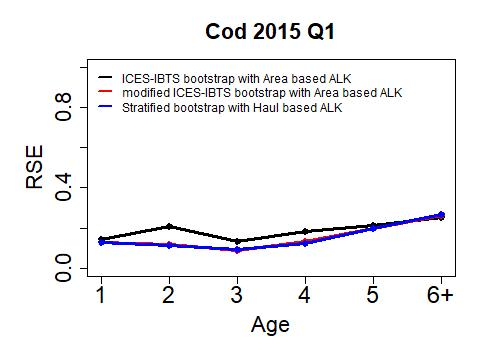
\includegraphics[width=0.33\textwidth]{figures/BootstrapMethodsPlots/CodAreaHaulAreaMod2015Q1.jpeg}} & \\
\subfloat[ ]{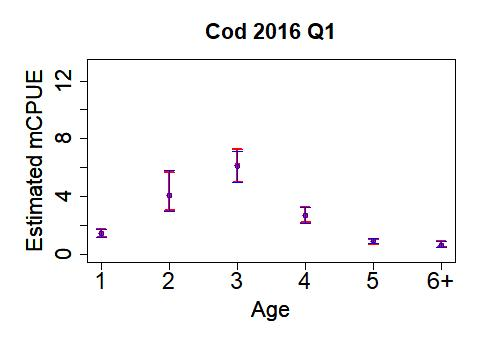
\includegraphics[width=0.33\textwidth]{figures/ALKplots/CodAreaHaulEstimates2016Q1.jpeg}} & 
\subfloat[]{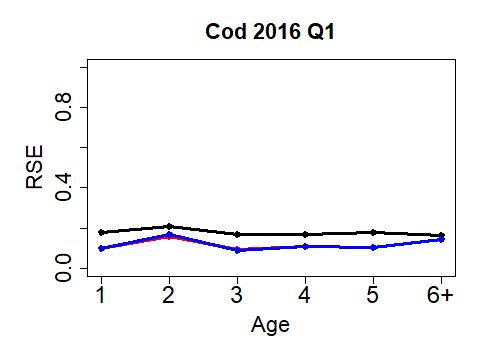
\includegraphics[width=0.33\textwidth]{figures/BootstrapMethodsPlots/CodAreaHaulAreaMod2016Q1.jpeg}} & \\
\subfloat[]{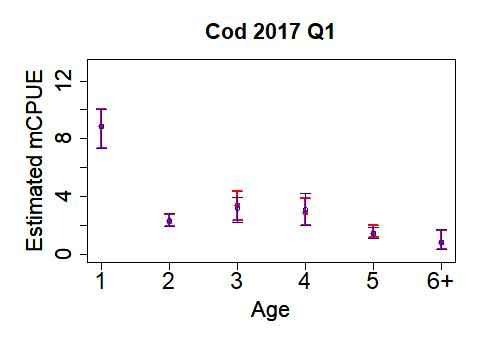
\includegraphics[width=0.33\textwidth]{figures/ALKplots/CodAreaHaulEstimates2017Q1.jpeg}} & 
\subfloat[]{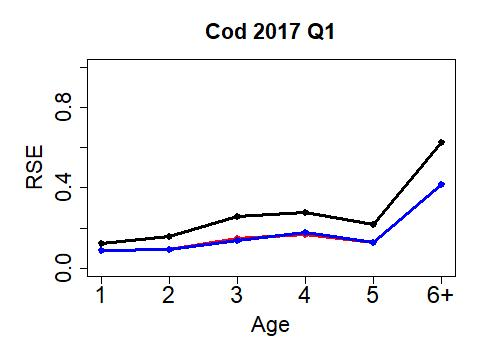
\includegraphics[width=0.33\textwidth]{figures/BootstrapMethodsPlots/CodAreaHaulAreaMod2017Q1.jpeg}} & \\
\subfloat[]{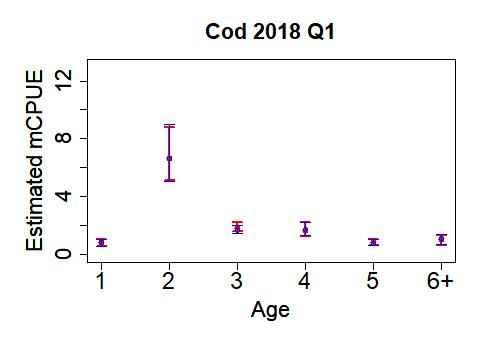
\includegraphics[width=0.33\textwidth]{figures/ALKplots/CodAreaHaulEstimates2018Q1.jpeg}} & 
\subfloat[]{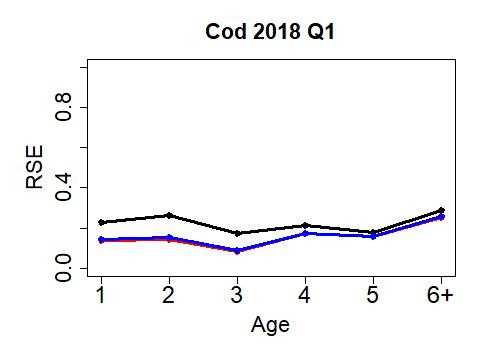
\includegraphics[width=0.33\textwidth]{figures/BootstrapMethodsPlots/CodAreaHaulAreaMod2018Q1.jpeg}} & \\
\end{tabular}
\end{figure*} 


\clearpage
%For North Sea Cod, one fish per 5cm length group width is sufficient to estimate age composition from trawl surveys (Figure \ref{fig:removal1OtolithCodQ1})
%While the current sampling strategy recommended by ICES for North Sea IBTS Cod is \textit{one} fish per 1cm length group width for age determination, some nations sampled more than \textit{one} fish per 1cm.
% This minor difference indicates that the current extensive age reading can be reduced with a minor loss.
\subsection{Evaluation of sampling strategy of otoliths}
\label{sec:optimumeffortresultsOtoliths}
In this section we investigate the effect of reducing effort, with respect to otolith collection, on the expected relative standard error (RSE) of estimated relative abundance-at-age of North Sea Cod (\ref{eq:abundanceestimatornorthsea}). For all experiments, we apply the haul based ALK and estimates are provided for 500 bootstrap replications. Firstly, we sample \textit{one} fish in length group widths: 5cm, 4cm, 3cm, 2cm, or 1cm for age determination (Figure \ref{fig:removal1OtolithCodQ1}).  In Figure \ref{fig:removal1OtolithCodQ1} we see that the difference in expected relative standard error is marginal, and this suggests that the current extensive age reading can be reduced with a minor loss. For age groups 1 to 4, little if any information in precision of mean catch per unit effort at age is achieved by reducing the length group width to 1cm. For age groups 5 and the plus group (6+), which accounts for a marginal proportion of the fish (Table \ref{PercentageAtAge2015-2018}), there is slight improvement in precision for shorter length group widths (e.g., 3cm, 2cm, or 1cm). This suggests that the length group width could be reduced to 1cm for longer fish, which are typically older, while maintaining a 5cm length group width for shorter fish. The higher variances in estimates of mean catch per unit effort in age groups 5 and and 6+ are largely driven by the relatively few trawl haul samples (Table \ref{PercentageAtAge2015-2018}) containing fish in these age groups. \\


\begin{small}
\begin{table}[h!]
\setlength\tabcolsep{3.5pt} 
\centering
\captionsetup{font=small, width = 12.2cm}{
\caption{Number of trawl hauls with age samples of North Sea Cod of age groups 5 and the plus group (6+) in years 2015-2018 quarter 1 (Q1). The number of fish measured for these age groups is also given (percentages are in parentheses). }\label{PercentageAtAge2015-2018}}
\begin{footnotesize}
\begin{tabular}{cccccccccc}
  \hline \\ [0.3ex]
{\bf Year}   & \multicolumn{2}{c}{\thead{\bf Number of hauls \\ \bf with age data }} & \multicolumn{2}{c}{\thead{\bf Number sampled \\ \bf at age }} & \multicolumn{1}{c}{\thead{\bf Total catch \\ \bf sampled for age }}  & \thead{\bf Total hauls \\ \bf with age samples} \\[0.8ex]
&   {age 5} & {age 6+}  & {age 5} & {age 6+}   \\ [0.5ex]
 \hline \\ [0.3ex]
	
{ 2015} & 45 (15\%) & 38 (13\%) & 103 (3.6\%) & 77 (2.7\%) &   2877 & 301\\[1ex]

{ 2016}  & 79 (33\%) & 56 (23\%) & 153 (7.5\%) & 97 (4.7\%) &  2044  & 243   \\[1ex]

{ 2017} & 86 (29\%) & 46 (16\%) & 194 (7.8\%) & 99 (3.5\%) &  2501   & 293 \\[1ex]

{ 2018} & 61 (27\%) & 45 (20\%) & 102 (6.4\%) & 124 (7.8\%) &  1596  & 229\\[0.8ex]

   \hline \\[0.1ex]
\end{tabular}
\end{footnotesize}
\end{table}
 \end{small}

Secondly,  we investigate the effect on expected relative standard error of the mean catch per unit effort at age of North Sea Cod if \textit{one}, \textit{two}, \textit{three}, \textit{four} or \textit{five} fish per 5cm length group width are sampled for age determination. Figure  \ref{fig:removalCod5cmQ1} confirms that one fish per 5cm is sufficient to estimate the age composition as the improvement in precision from sampling more than one fish per 5cm length group width is marginal. A similar trend is observed in the third quarter in 2015-2018 and these results are presented  in Supplementary Materials \ref{secAp:evalutionofotoliths}. Table \ref{resamplingOtoliths2015-2018} gives the average number of fish sampled for age in each length group width  for 500 bootstrap replicates (percentage of fish sampled are in parentheses). In all years and quarters, at most 51\% of fish sampled for age determination are in length group width 5cm (Tables \ref{resamplingOtoliths2015-2018} and \ref{resamplingOtoliths2015-2018Q3} in Supplementary Materials \ref{secAp:evalutionofotoliths}). \\

\begin{small}
\begin{table}[h!]
\setlength\tabcolsep{6.5pt} 
\centering
\captionsetup{font=small, width = 15.5cm}{
\caption{Average number of fish sampled for age determination from 500 bootstrap replicates in length group widths: 5cm, 4cm, 3cm, 2cm or 1cm (percentages are in parentheses). In each bootstrap replicate \textit{one} fish is sampled for age determination in each length group width in the first quarter in 2015-2018. Also, \textit{one}, \textit{two},  \textit{three},  \textit{four}  or \textit{five} fish are sampled in a 5cm length group width and the average number is given.  The total number of fish sampled in a given year of interest in IBTS is also given.}\label{resamplingOtoliths2015-2018}}
\begin{footnotesize}
\begin{tabular}{clclclclclclclclclclclclclclclclclclclclclclclclclclcl}
  \hline \\ [0.3ex]
{\bf Year}   & \multicolumn{5}{c}{\bf Length group width  } & \thead{\bf Total ages sampled \\ \bf in Q1 in the given year }  \\[0.8ex]
&   {5cm} & {4cm}  & {3cm} & {2cm}  & {1cm} \\ [0.5ex]
 \hline \\ [0.3ex]
	
{ 2015} & 1166 (40\%) & 1278 (43\%) & 1457 (50\%) & 1714 (58\%) &  2185 (75\%)   & 2895\\[1ex]

{ 2016}   &997 (49\%) & 1092 (54\%) & 1229 (61\%) & 1409 (70\%) &  1743 (86\%)   &2046\\[1ex]

{ 2017} & 1183 (47\%) & 1297 (51\%) & 1465 (58\%) & 1722 (68\%) &  2178 (87\%)   &2501\\[1ex]

{ 2018}  & 804 (51\%) & 881 (56\%) & 980 (63\%) & 1132 (72\%) &  1350 (86\%)   &1600\\[2.5ex]

{\bf Year} & \multicolumn{5}{c}{\bf Number of fish sampled for age per 5cm length group width} & \\[1.2ex]
& 1 & 2 & 3 & 4 & 5 \\
\cmidrule(lr{0.3em}){2-6} \\ [0.5ex]%
2015 & 1166 (40\%) & 1705 (58\%)& 2033 (69\%)& 2271 (77\%)&2423 (82\%) & 2895 \\ [1ex]
2016 &997 (49\%) &1421 (70\%) & 1660 (82\%)&1793 (88\%) & 1872 (91\%)& 2046& \\ [1ex]
2017 &1183 (47\%) & 1727 (69\%) & 2035 (81\%)& 2225 (88\%) & 2331 (92\%)& 2501&  \\ [1ex]
2018 &804 (51\%) & 1127 (72\%)&1307 (83\%) & 1403 (89\%)& 1460 (93\%) &  1600 \\ [1ex]

   \hline \\[0.1ex]
\end{tabular}
\end{footnotesize}
\end{table}
 \end{small}
 

%The expected RSE with all the fish sampled for North Sea Cod is represented by the horizontal lines.
\clearpage
\begin{figure*}[h!]
\centering
\captionsetup{font=small, width = 16.5cm}{
\caption[]{Expected relative standard error of the mean catch per unit effort at age of North Sea Cod in Q1 in years 2015-2018 with different length group widths for 500 bootstrap samples. We sample \textit{one} fish in the following length group widths: 5cm, 4cm, 3cm, 2cm or 1cm, which is represented by the squares.  The numbers 1 through 6+ (and associated colours) represent the age of Cod, where 6+ is all fish of age 6 or older.}\label{fig:removal1OtolithCodQ1}}
\begin{tabular}{@{}ccc@{}}
\subfloat[]{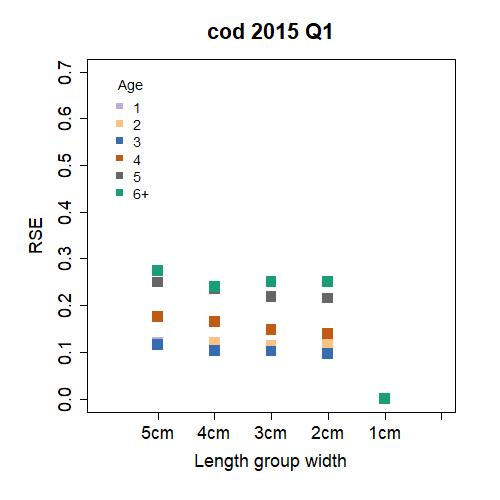
\includegraphics[width=0.42\textwidth]{results/olav/resamplingOtoliths/removalcod2015Q1.jpeg}} & 
\subfloat[]{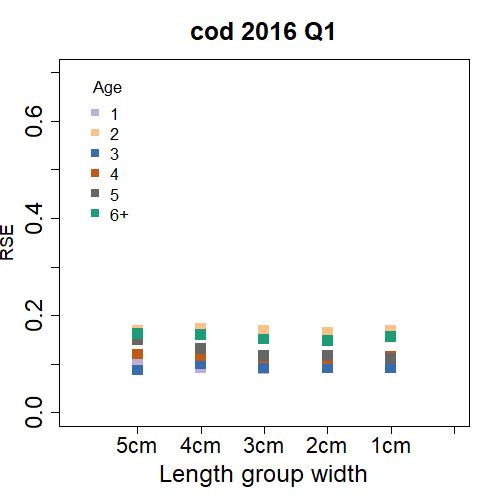
\includegraphics[width=0.42\textwidth]{results/olav/resamplingOtoliths/removalcod2016Q1.jpeg}} & \\
\subfloat[]{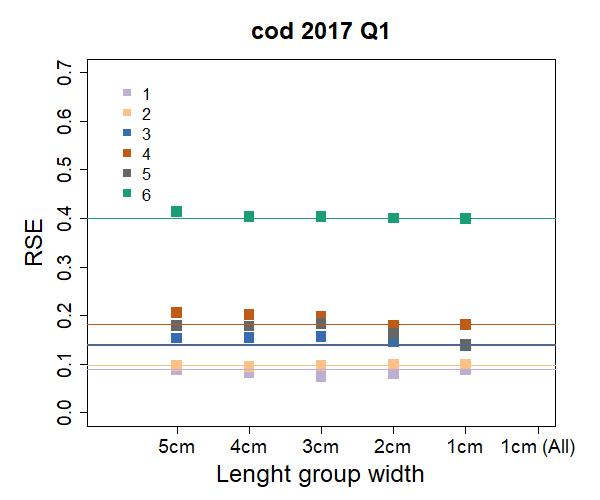
\includegraphics[width=0.42\textwidth]{results/olav/resamplingOtoliths/removalcod2017Q1.jpeg}} & 
\subfloat[]{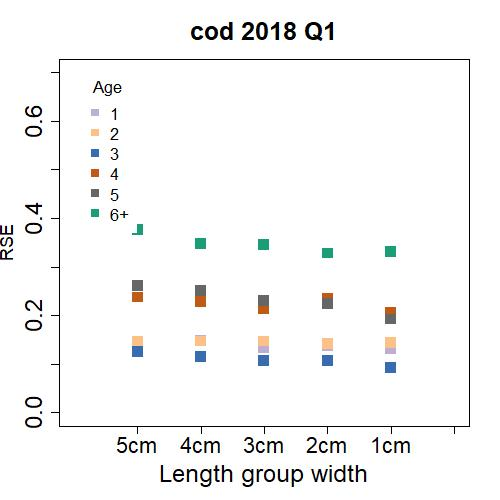
\includegraphics[width=0.42\textwidth]{results/olav/resamplingOtoliths/removalcod2018Q1.jpeg}} & 
\end{tabular}
\end{figure*} 

\clearpage
\begin{figure*}[h!]
\centering
\captionsetup{font=small, width = 16.5cm}{
\caption[]{Expected relative standard error of the mean catch per unit effort at age of North Sea Cod in Q3 in years 2015-2018 for varying number of fish sampled for age in a 5cm length group width: \textit{one}, \textit{two}, \textit{three}, \textit{four} or \textit{five} fish sampled for age determination is represented by the squares.  The expected RSE for all fish currently sampled per length group in the North Sea, denoted by ``c", is represented by the circle. The current sampling strategy recommended by ICES from 2018 Q1 for North Sea Cod is \textit{one} fish per 1cm length group width from each trawl haul, although some nations sampled more than one fish for age determination per 1cm length group width. estimates are provided for 500 bootstrap replicates}\label{fig:removalCod5cmQ1}}
\begin{tabular}{@{}ccc@{}}
\subfloat[]{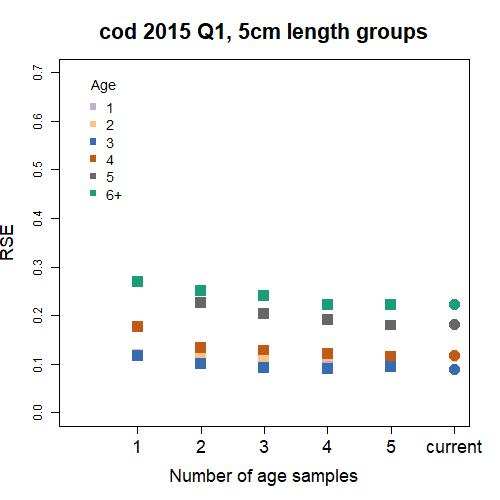
\includegraphics[width=0.42\textwidth]{results/olav/resamplingOtoliths/removalcod2015Q1DL5.jpeg}} & 
\subfloat[]{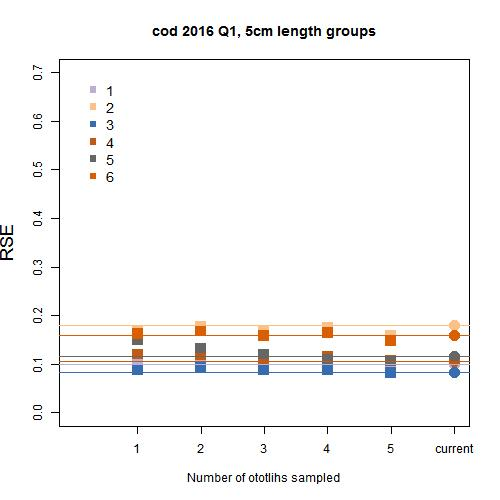
\includegraphics[width=0.42\textwidth]{results/olav/resamplingOtoliths/removalcod2016Q1DL5.jpeg}} & \\
\subfloat[]{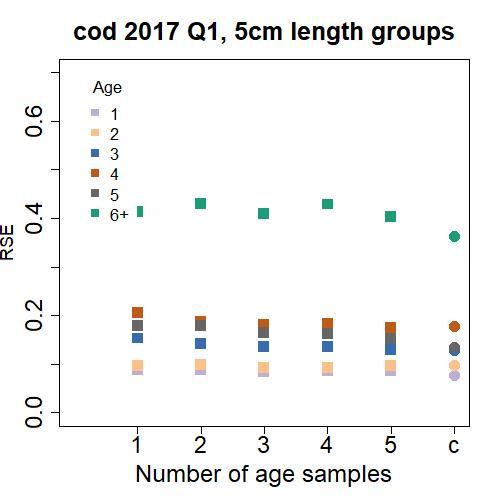
\includegraphics[width=0.42\textwidth]{results/olav/resamplingOtoliths/removalcod2017Q1DL5.jpeg}} & 
\subfloat[]{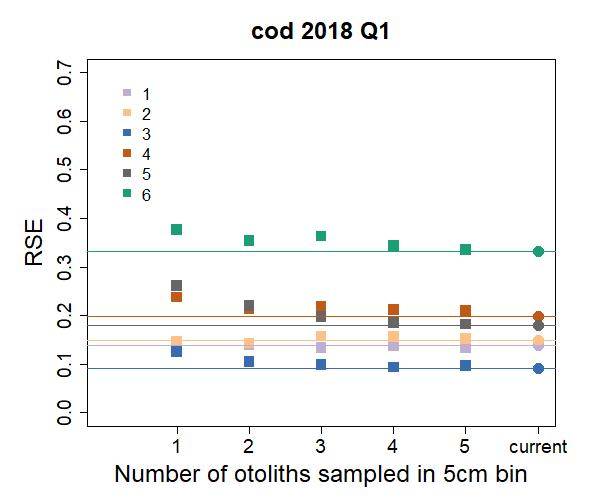
\includegraphics[width=0.42\textwidth]{results/olav/resamplingOtoliths/removalcod2018Q1DL5.jpeg}} & 
\end{tabular}
\end{figure*} 


\clearpage
\subsection{Evaluation of sampling strategy of otoliths and hauls}
\label{sec:optimumeffortresultsHaul}

%\natty{(I think this needs clarification. The argument seems to me to suggest that there is little gain in adding stations, and I might need clarification on how to interpret the asymptotic limit of sampling with replacement from a finite data set. See additional comments in other attachment.)}\\

In this section we investigate the effect on the expected relative standard error on the mean catch per unit effort at age if \textit{one} or \textit{five} fish  per 5cm length group width from each trawl haul are sampled for age determination. In the resampling procedure, we set the total number of trawl hauls in the study area, $╛N =  50, 75, 100, 150, 200, 300, 400 \ \mathrm{or} \  500$ such that the proportion of hauls in the round fish areas (RFAs) is the approximately the same as a real survey design (see Section \ref{sec:evaluatingtrawlhauls}), and no fewer than two hauls are taken in a RFA.  For each experiment, 500 bootstrap replicates are taken and the expected relative standard error from the area based ALK is computed.  Figures \ref{OtolithHauls2015-2016Q1} and  \ref{OtolithHauls2017-2018Q1} present the expected relative standard error for the estimated mean catch per unit effort at age of North Sea Cod in years 2015-2018 Q1. 

At least 345 trawl hauls are sampled in the years of interest at the North Sea International Bottom Trawl Surveys (Table \ref{tab:realdata2017-2018Cod}), but as shown in Figures \ref{OtolithHauls2015-2016Q1} and  \ref{OtolithHauls2017-2018Q1}, there is little gain in increasing the number of trawl hauls ($>$ 300). If the number of trawl hauls is reduced ($< 300$) however, the expected relative standard error, particularly for older Cod increases quickly, which indicates that gains can still be had by sampling more hauls. The analyses further show that  there is no real difference in expected relative standard error if one or five fish are sampled in a 5cm length group width, supporting the recommendation that \textit{one} fish per 5cm length group width per trawl haul is sufficient for age determination. We conduct analysis for the third quarter (Q3) in 2015-2018 and several more earlier years (1997-1999) for which more older North Sea Cod were caught, with similar results (Supplementary Materials \ref{secAp:evalutionofotolithsAndHauls}). Furthermore, analyses using the haul based ALK (although not shown) gave similar results.

%The analyses further show that the subsample sizes of otoliths per 5cm length group width from each trawl haul has minimal effect on precision supporting the recommendation for sampling \textit{one} fish per 5cm length group width from each trawl station for age determination. We conduct analysis for the third quarter (Q3) in 2015-2018 and several more earlier years (1997-1999) for which more older North Sea Cod were caught, with similar results (Supplementary Materials \ref{secAp:evalutionofotolithsAndHauls}). Furthermore, analyses using the haul based ALK (although not shown) gave similar results.}
 

\clearpage
\begin{figure*}[h!]
\centering
\captionsetup{font=small, width = 16.5cm}{
\caption[]{Expected relative standard error (RSE) for North Sea Cod in years 2015-2016 Q1 when sampling \textit{one} (red line) or \textit{five} (black line) fish in length group width 5cm  for age determination from each trawl station for 500 bootstrap samples. For each sampling strategy of otoliths, the area based ALK is used for the given number of hauls, $N =50, 75, 100, 150, 200, 250, 300, 350, 400 \  \mathrm{or} \ 500$. The age of North Sea Cod ranges from 1 to 6 where 6+ is a plus group consisting of all fish of age 6 or older. }\label{OtolithHauls2015-2016Q1}}
\begin{tabular}{@{}ccc@{}}
\subfloat[]{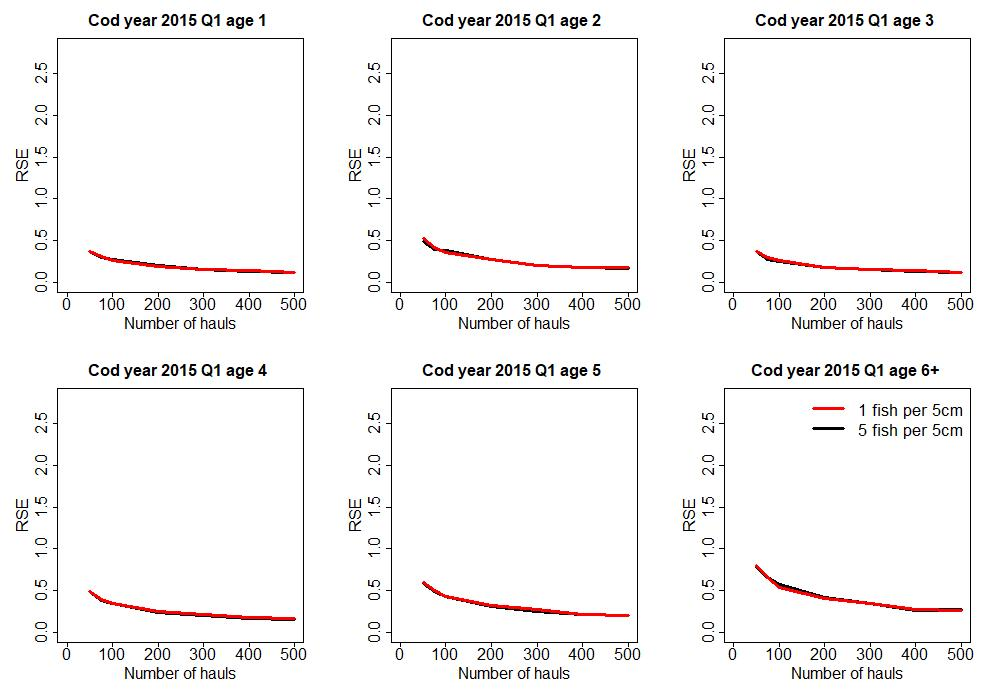
\includegraphics[width=0.85\textwidth]{results/olav/resamplingNandotoliths/resampleNandOcod2015Q1DL5datras.jpeg}} & \\
\subfloat[]{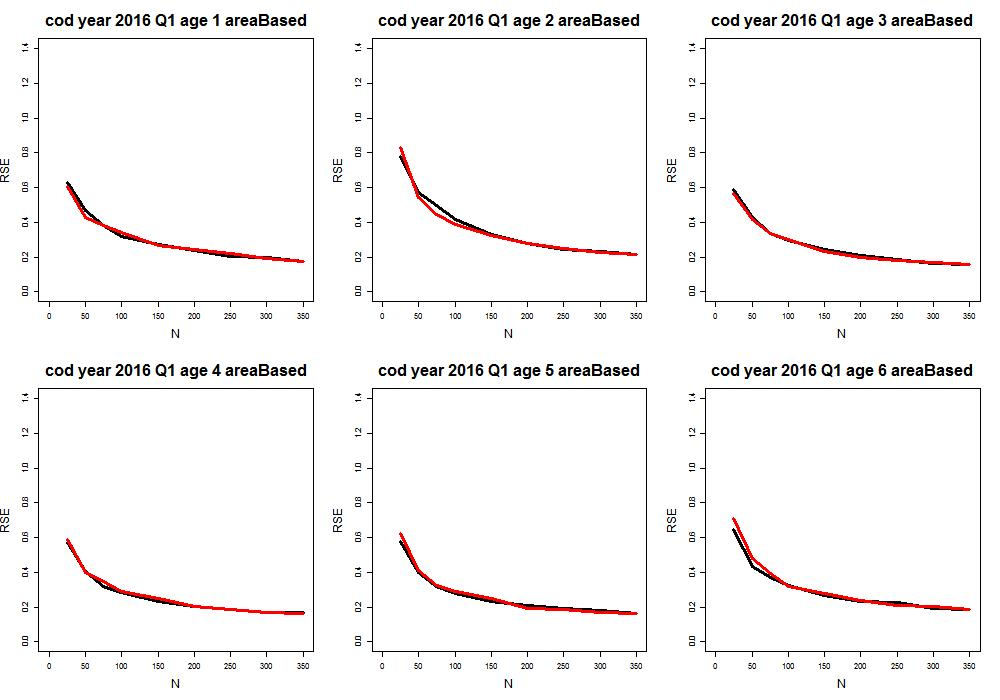
\includegraphics[width=0.85\textwidth]{results/olav/resamplingNandotoliths/resampleNandOcod2016Q1DL5datras.jpeg}} & 
\end{tabular}
\end{figure*} 


\clearpage
\begin{figure*}[h!]
\centering
\captionsetup{font=small, width = 16.5cm}{
\caption[]{Expected relative standard error (RSE) for North Sea Cod in years 2017-2018 Q1 when sampling \textit{one} (red line) or \textit{five} (black line) fish in length group width 5cm  for age determination from each trawl station for 500 bootstrap samples. For each sampling strategy of otoliths, the area based ALK is used for the given number of hauls, $N = 50, 75, 100, 150, 200, 250, 300, 350, 400 \  \mathrm{or} \ 500$. The age of North Sea Cod ranges from 1 to 6 where 6 is a plus group consisting of all fish of age 6 or older.  }\label{OtolithHauls2017-2018Q1}}
\begin{tabular}{@{}ccc@{}}
\subfloat[]{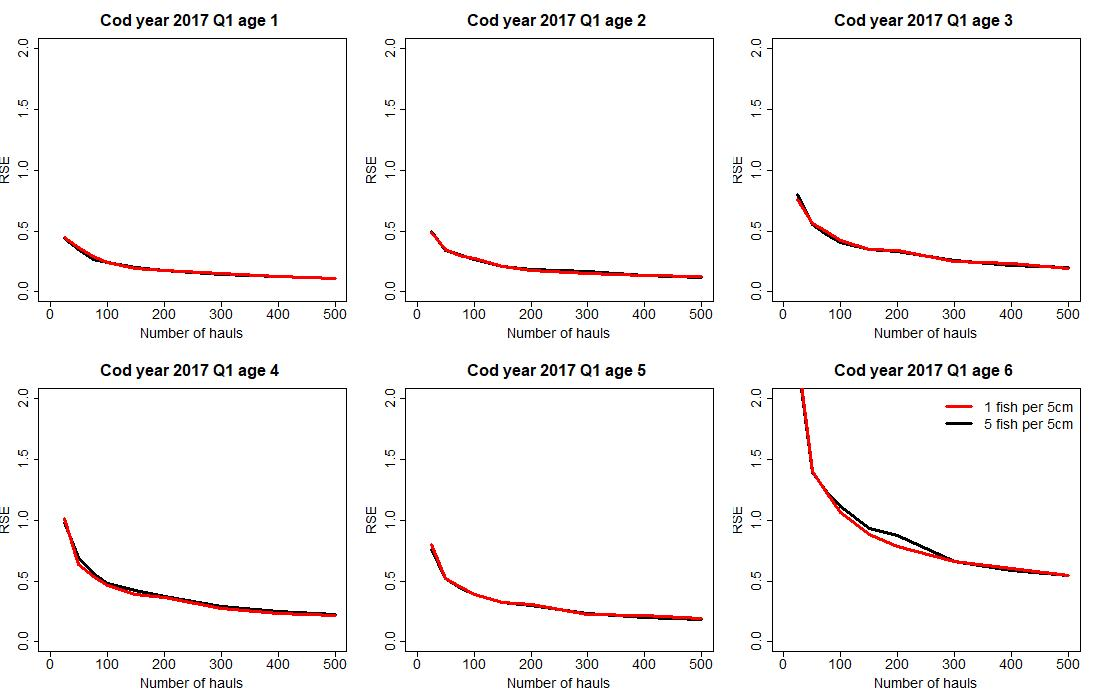
\includegraphics[width=0.85\textwidth]{results/olav/resamplingNandotoliths/resampleNandOcod2017Q1DL5datras.jpeg}} & \\
\subfloat[]{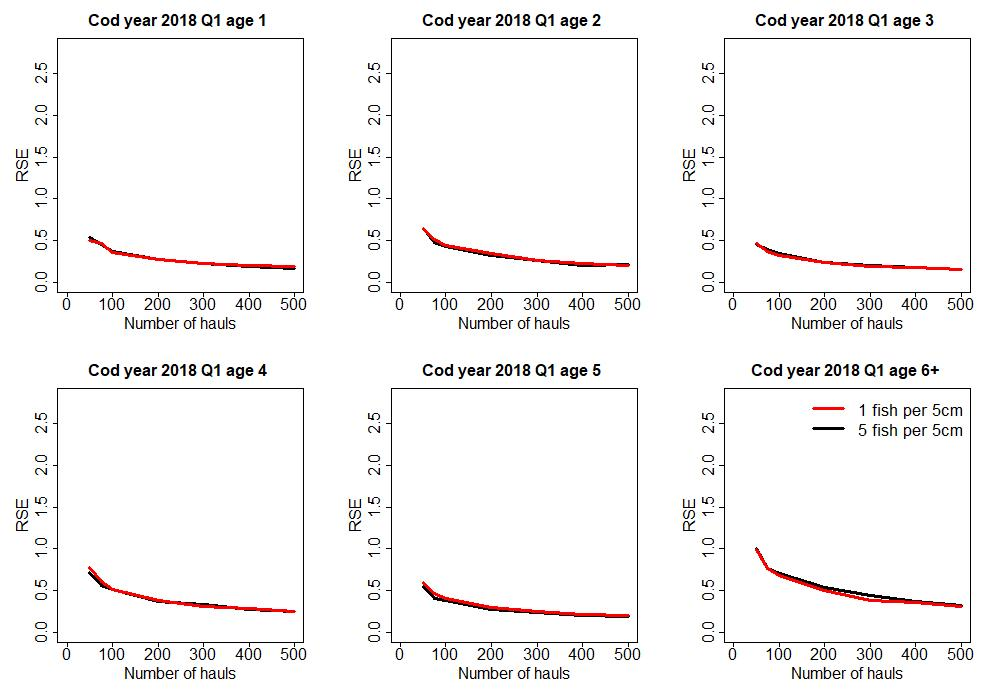
\includegraphics[width=0.85\textwidth]{results/olav/resamplingNandotoliths/resampleNandOcod2018Q1DL5datras.jpeg}} & 
\end{tabular}
\end{figure*} 


\clearpage
\section{Discussion}
\label{sec:discussion}


We have developed estimators and bootstrap procedures that differ slightly from those previously proposed for these data. 
Our intention has been to better align the design of estimators with the design of the sampling for both the ALK definitions and the resampling procedures. In particular, this better reflects the spatial structure of the sampling, taking into account any spatial variation in age-length relationships. For the particular examples we have analysed, the 
differences between the expected RSE estimates for different ALKs and resampling-schemes are small with respect to common interpretation. \natty{For the estimator where coarse spatial representation is employed in both the ALK and the bootstrap, the estimated RSE is deviating consistently from the alternatives we propose.}

Faithfully mimicking the sampling design is not only useful for bootstrap estimates, but also allows us to estimate the effect of reducing sampling effort. For age sample collection,  consideration of what effort is necessary is a pressing issue as age-reading is a demanding skill to develop and trained  age-readers is a resource shared with other surveys, and potentially other species. Strained age-reading capacity prohibits development of new surveys, and may introduce unfortunate bias in otherwise unbiased samples, if otoliths are not all read before advice is due. We therefore performed an analysis mimicking reduced otolith sampling. We have presented a range of options for less intensive otolith-sampling to which the variance of abundance-at-age estimates are highly robust. We have in this respect been conservative in what options we have explored, and limited ourselves to sampling-reductions that appear to essentially preserve precision, and thus not alter the usability of estimates. We find it important in that regard to not compromise on primary sampling units, and have considered only sampling protocols that sample the target  species the same way at all stations. We do however note that the variance of older fish has a larger response to sample reductions than smaller fish, so that reductions in sampling is best considered first for short length-strata.
 
More aggressive sample-reductions could extend beyond the criteria of essentially keeping the same precision. 
Such analysis could be performed by coupling the resampling analysis to the effect of downstream use, such as stock-assessment. 
An important caveat in that respect is that results will be very sensitive to the choice of stock-assessment model, which 
after all are typically subject to change during the lifetime of a survey time-series.

For routine International Bottom Trawl Surveys of the North Sea Cod, the number of fish sampled for age determination could be reduced   by at least  50\% without appreciable loss of precision in abundance-at-age estimates.  This could free up resources from a heavily strained age-reading staff and avoid bias introduced by incomplete readings in thus survey or in other data 
collection programs competing for the same age reading capabilities.

%The time saved by collecting and reading fewer otoliths  is significant.
%We conclude from this work that 


%\emph{I think we should conclude with 
%some numbers. which I don't have right now E.g. for the case of cod we find that the total number of otoliths can effectively
% be reduced by x\%, without appreciable loss of precision in abundance-at-age estimates. This could free up resources from a
% heavily strained age-reading staff and avoid bias introduced by incomplete readings in thus survey or in other data 
%collection programs competing for the same age reading capabilities.}

%
%\clearpage
%\begin{enumerate}
%\item \nat{I also think we should highlight that the effort regarding reading otoliths is a real resource problem for IMR, perhaps with a personal communication reference.  And that our work share light on that the reduction can be performed with minor loss.}
%
%\item \nat{Perhaps we can discuss that the age reduction seems to have a larger effect on the older cod. And that this is intuitive reasonable since the age is more uncertain among the larger fish.}
%
%\item \nat{I think we should write something about that the reduction of age sampling could be further investigated by investigating changes in assessment. And state that this is not conducted in our work.} 
%\end{enumerate}
%
%
%\begin{enumerate}
%\item \natty{Highlight main point from introduction}
%\item \natty{propose a recommendation for ALK or bootstrap approach}
%\item \natty{Recapitulate the different biases in area-based ALK, refer to result in Figure 3 and recommend our variants of ALK and bootstrap as these handles identified biases and we have shown that it makes some difference.}
%
%\item \natty{I agree with Olav that we can not demonstrate empirically that our suggestion is better, but we could still argue based on how it is design to eliminate these biases.}
%
%\begin{itemize}
%\item  \natty{Recapitulate the importance of reducing age reading effort, and argue for larger length groups to be considered for sampling manuals. I am not thinking a classic cost-benefit argument, but rather arguing that:}
%
%\begin{enumerate}
%\item \natty{Overloaded age-reading staff may introduce bias by the order the read ages if they cannot finish the age reading timely.}
%
%\item \natty{Freeing up age-reading capacity may allow us to redistribute effort to reading other species.}
%\end{enumerate}
%
%\end{itemize}
%
%\item \natty{Figures: This should be considered a minor point.}
%
% \item \natty {I don't want to impose additional figure work at this point, but in case we have one laying around I'll mention it anyway. I would be interested in including one example where we take the sampling regimes to some extreme (like very wide length-groups), just to confirm to a sceptically inclined reader that the RSE does actually go up at some point.}
%\end{enumerate}
%
%\subsection*{\normalsize Evaluation of ALK estimators and borrowing of ALKs}
%In this research we present estimators for age composition and sampling strategies for age determination, which are based on multistage trawl sample surveys in the North Sea. We show that the estimator for mean catch per unit effort at age based on \ed{(constant?)} ALKs over relatively large areas is equivalent to that based on a spatial designed-based ALK provided that the variability in the ALK is included in the estimation process. However, spatial ALKs \citep{berg2012spatial, gerritsen2006simple, hirst2012bayesian} are more favorable as regional differences in ALKs may exist, and borrowing of ALKs between regions would introduce bias  \citep{aanes2015efficient,kimura1977statistical}. 
%
%In multistage bottom trawl surveys, larger samples of length distribution are collected while only a small fraction of the catch with length measurements are analysed for age. Therefore, ALKs are often borrowed, for example from another station (or haul), stratum or time period, to fill gaps. In our North Sea Cod case study, the primary sampling unit is the trawl haul and sampling is stratified at the \ed{second stage} with respect to statistical rectangles and at the \ed{third stage}, with respect to round fish areas. In the years of interest for this research, at most 1\%  of fish measured for lengths across round fish areas had missing age data, while 15\% across hauls had missing age data. In our proposed haul based ALK estimator, borrowing of ALKs is done between length groups within hauls or, if possible, across hauls at a maximum distance of 60 nautical miles. If these possibilities are not practical the area based ALK is implemented. Although this has minor effect on the estimated relative abundance-at-age (small proportion of lengths without age data), the efficiency of the estimators can be improved with the use of model-based methods that are based on poststratification \citep{holt1979post, valliant1993poststratification} or without stratification \citep{berg2012spatial, berg2014evaluation}.  
%
%Estimates of precision of relative abundance-at-age based on these ALK estimators can be obtained using bootstrapping methods that replicate the complex multistage survey design, but these would require access to data on age and length compositions at the haul level. In terms of which bootstrap procedure (that replicate the multistage survey design) is best, it is difficult to say but by using these bootstrap methods to create input data in a statistical assessment model, as in \citep{berg2014evaluation}, precision to estimates of spawning stock biomass and fishing mortality can be quantified and the best approach may be determined.
%
%
%%(\ed{did we actually do this step? I thought Sondre and Jon Helge said to stop if this happens. Alternatives are 1) model base approach or removing areas from the study where ages are lacking. Because if we do this, we are implementing exactly what DATRAS did}). \olav{We currently do this step. This step is done for relatively few fish. I suggest we argue that this step has minor effect on the estimate by illustrating the portion of fish which are mapped from length to age by this step. We can delete those areas, but then I think there is a loot of pitfalls to get into. I suspect these hauls are in areas with little catch of the species of interest, and care must be taken if deleting those areas/hauls without getting biased estimates.}
%
%
%\subsection*{\normalsize Evaluation of sampling strategies for age determination based on empirical data}
%%\subsubsection*{Reducing the number fish sampled for otoliths}
%%\subsubsection*{Reducing or increasing the number of hauls }
%
%
%\subsection*{\normalsize Conclusions}
%\label{sec:conclusion}
%
%
%\clearpage   
%
%\begin{enumerate}
%\item I also think we should highlight that the effort regarding reading otoliths is a real resource problem for IMR, perhaps with a personal communication reference.  And that our work share light on that the reduction can be performed with minor loss.
%
%\item Perhaps we can discuss that the age reduction seems to have a larger effect on the older cod. And that this is intuitive reasonable since the age is more uncertain among the larger fish.
%
%\item I think we should write something about that the reduction of age sampling could be further investigated by investigating changes in assessment. And state that this is not conducted in our work. 
%
%\item Good, then we do the experiment with N larger or equal 50.
%
%\item Perhaps a justification can be that the area based ALK is typically used for producing indices. At least I have understood it so that it is the area based ALK is mostly used. A justification for using haul based is that we then try to accommodate for possible haul to haul variation.
%
%\item The sampling procedure described on page 10-11 is correct. We do not need to adjust the sampling procedure if we use haul based ALK. We sample hauls stratified wrt RFA with replacement, and the ages with the pseudo boostrap procedure. After we have simulated one realization, we can use both the area based and haul based ALK. Did this answer your questions?
%
%\item Since Jon Helge said we should use the area based ALK we can use that. I do not see the reason why we should not use the haul based ALK. The reason I also ran with haul based ALK was just because I wanted to see what happened, and we get approximately the same results. We can perhaps include in the paper that ”We also ran the simulation experiment with hauls based ALK, and it did not change the conclusions (not shown)”.
%
%\item I see that with N = 25 we sometimes get fewer than 2 hauls in an RFA (in RFA 5 and 9).   That newer happen when we sample 50 hauls or more in any of the years 1997-1999 or 2015-2018. Sorry I did not see this before, I thought I had implemented the program such that it would stop if that scenario occurred and in that case I could look into the details how to treat such a scenario if it was needed. I suggest we do not sample 25 hauls and stop at 50. There seems to be much noise when we sample 25 hauls also, such that we should increase the number of bootstrap samples in that case also to get a good estimate of the expected RSE. In case we want to sample 25 hauls we need to decide on a procedure to choose which RFA we sample fewer hauls from such that the number of hauls is 2 or larger for every RFA. I think this is details and we should just stop at 50, it does not change any of the results of the experiment. Do you have any opinions regarding this?
%
%%(\ed{did we actually do this step? I thought Sondre and Jon Helge said to stop if this happens. Alternatives are 1) model base approach or removing areas from the study where ages are lacking. Because if we do this, we are implementing exactly what DATRAS did}). \olav{We currently do this step. This step is done for relatively few fish. I suggest we argue that this step has minor effect on the estimate by illustrating the portion of fish which are mapped from length to age by this step. We can delete those areas, but then I think there is a loot of pitfalls to get into. I suspect these hauls are in areas with little catch of the species of interest, and care must be taken if deleting those areas/hauls without getting biased estimates.}
%
%%extensive samples of length distribution are available, while age samples are unavailable for 
%%
%%In our spatial ALK estimator  \\
%%
%%%as regional differences in ALKs may exist, resulting in bias when borrowing of ALKs between regionsis done
%%%& Cod with missing age in RFAs     & 0.30\%& 0.13\% & 0.13\% & 0.34\% & 0.68\% &  0.07\% & 0.51\%  & 0.11\%  \\[1ex]  
%%%& Cod with missing age in hauls    & 10.06\% & 14.20\% & 6.18\%& 6.32\% & 2.25\% &0.27\%   & 1.40\%   & 0.77\% \\[0.1ex] 
%%%& $\% \mathrm{length \ groups}$ with missing ages in RFA      &  &  0.03 \% &   &   \\[1.5ex]  
%%%& $\% \mathrm{length \ groups}$ with missing ages in haul     &  &   0.03 \% &   &   \\[0.5ex]
%%
%%
%%\begin{itemize}
%%\item Spatial structures in the ALK have also been investigated in \citet{berg2012spatial} and  \citet{hirst2012bayesian}. 
%%\item As differences in age-length structures may exist over large areas, these differences do have the potential to result in a biased ALK \citep{gerritsen2006simple,kimura1977statistical}. To account for the spatial distribution we propose a design-based ALK that is haul dependent (Section \ref{sec:haulestimator}).
%%\end{itemize}
%\end{enumerate}


\clearpage

%
%
%\begin{figure*}[h!]
%\centering
%\begin{tabular}{@{}ccc@{}}
%\subfloat[]{\includegraphics[width=0.79\textwidth]{figuresNotUsed/AgeAndLengthHaulRFA4Cod2018Q1.jpeg}} &\\
%\subfloat[]{\includegraphics[width=0.99\textwidth]{figuresNotUsed/AgeAndLengthHaulRFA8Cod2018Q1.jpeg}} & 
%\end{tabular}
%\captionsetup{font=small, width = 14.5cm}{
%\caption[]{ }\label{AgeLengthHauls}}
%\end{figure*} 
%
%
%
%\clearpage
%
%\begin{figure*}[h!]
%\centering
%\begin{tabular}{@{}ccc@{}}
%\subfloat[]{\includegraphics[width=0.79\textwidth]{figuresNotUsed/AgeAndLengthHaulRFA5Cod2018Q1.jpeg}} &\\
%%\subfloat[]{\includegraphics[width=0.99\textwidth]{figuresNotUsed/AgeAndLengthHaulRFA8Cod2018Q1.jpeg}} & 
%\end{tabular}
%\captionsetup{font=small, width = 14.5cm}{
%\caption[]{ }\label{AgeLengthHauls}}
%\end{figure*} 








\clearpage

\bibliographystyle{apalike}
\bibliography{BibliographyIbts}

\clearpage


\begin{center}
\textbf{\Large Supplemental Materials: An Analysis of the North Sea International Bottom Trawl Survey.}
\end{center}
%%%%%%%%%% Merge with supplemental materials %%%%%%%%%%
%%%%%%%%%% Prefix a "S" to all equations, figures, tables and reset the counter %%%%%%%%%%
\setcounter{section}{0}
\setcounter{equation}{0}
\setcounter{figure}{0}
\setcounter{table}{0}
\setcounter{page}{1}
\makeatletter
\renewcommand{\thesection}{S\arabic{section}}
%\renewcommand{\theequation} {\arabic{section}. S\arabic{equation}}
%\renewcommand{\theequation}{S\arabic{equation}}
\renewcommand{\theequation}{S\arabic{section}.\arabic{equation}}
\renewcommand{\thefigure}{S\arabic{figure}}
\renewcommand{\bibnumfmt}[1]{[S#1]}
\renewcommand{\citenumfont}[1]{S#1}

\setcounter{table}{0}
\numberwithin{table}{section}
%\clearpage


\section{\large Areas fished by different countries in the North Sea IBTS}
\label{secAp:areasfishedappendix}
Typically, two countries fish each rectangle so that at least two trawl hauls are made per rectangle. However, intensified sampling is carried out in the following areas: at least 3 hauls per rectangle are taken in statistical rectangles  31F1, 31F2, 32F1, 33F4, 34F2, 34F3, 34F4, 35F3, 35F4; while six or more hauls per rectangle are taken in statistical rectangles  30F1, 32F2, 32F3, 33F2, 33F3 (ICES 1999).  The Skagerrak and Kattegat is fished solely by Sweden, who sample more than once in every rectangle while the west of Shetland (in Q1 and Q3) and inshore areas (Q3) is fished solely by Scotland. The edge of the Norwegian Trench is fished solely by Norway, but inshore areas near Denmark is fished by Denmark. The southern North Sea is fished by Denmark, Germany and England. France, typically, is the only country that surveys the western English Channel. Areas are surveyed by a single country because of the large proportion of untrawalable area (and subsequent gear damage issues experienced by other nations)  for efficient logistical purposes. Table \ref{countries} gives the countries and research vessels participating the North Sea IBTS.\\
\begin{small}
\begin{table}[h!]
\centering
\captionsetup{font=small, width = 15.5cm}{
\caption{Survey countries, vessel name, and period research vessels participating in first quarter (Q1) and third quarter (Q3) during 1997-2017.}\label{countries}}
\begin{tabular}{cccccccc}
\hline \\[0.1ex]
  & \multicolumn{2}{c}{\bf First Quarter (Q1)} & \multicolumn{2}{c}{\bf Third Quarter (Q3)}\\[1.5ex]
{\bf Country }  & Vessel name & Period    & Vessel name & Period  \\[0.5ex]
\hline \\[0.5ex]
Denmark  &   Dana   &   January-February  & Dana & July-August    \\[1ex]
France  & Thalassa II & January-February & - & -   \\[1ex]
Germany   &  Walther  Herwig III & January-February   &   Walther  Herwig III & July-August \\[1ex]
Netherlands &  Tridens 2 &  January-February   & - & -     \\[1ex]
Norway  &   G.O. Sars  & January-February &    Johan Hjort  & July   \\[1ex]
UK England &- & -&  Endeavour &  August-September  \\[1ex]
UK Scotland   &  Scotia III &  January-February & Scotia III &  July-August \\[1ex]
Sweden  &  Dana &  January-February  &  Dana &  August                  \\[0.5ex]
\hline
\end{tabular}
\end{table}
\end{small}




%\clearpage
\section{\large Otolith sampling per fish species}
\label{secAp:otolithappendix}
From 1991-2017, most countries conducted quota sampling of otoliths for age determination per length group in a RFA. But from 2013, Norway, Scotland and the Netherlands have been sampling one otolith per length class from each trawl haul. From 2018 Q1, all countries are required to sample one otolith per length class per trawl haul.  Table \ref{tab:otolithsTable} gives the minimum sampling levels of otoliths for the target species.\\ %However, for the smallest size groups, that presumably contain only one age group, the number of otoliths per length class may be reduced, and more otoliths per length are required for the larger length classes.\\ %\\
%\clearpage
\begin{small}
\begin{table}[h!]
\centering
\caption{Minimum sampling levels of otoliths by species for RFA or per trawl haul.}
\label{tab:otolithsTable}
\begin{tabularx}{\linewidth}{r l l l l X}
\toprule 
Period &  Species  & Minimum sampling levels of otoliths per length class    \\[0.7ex]
\midrule \\[0.1ex]
{\bf 1991-2017} & & {\bf Number of otoliths per length class in a RFA}  \\[1.0ex]
     & herring  &  $8$  otoliths per $\frac{1}{2}$ cm group \\[0.5ex]
     & sprat    & $16$  otoliths per $\frac{1}{2}$ cm length class  $8.0 -11.0$ cm\\[0.5ex]
              & & $12$  otoliths per $\frac{1}{2}$ cm length class  $\geq 11.0$ cm\\[0.5ex]
& mackerel      & $8$  otoliths per $\frac{1}{2}$ cm length class \\[0.5ex]
& Cod       	  & $8$  otoliths per $1$ cm length class\\[0.5ex]
&haddock   	  & $8$  otoliths per $1$ cm length class \\[0.5ex]
&whiting    	  & $8$  otoliths per $1$ cm length class \\[0.5ex]
&Norway pout   & $8$  otoliths per $1$ cm length class\\[0.5ex]
&Saithe        & $8$  otoliths per $1$ cm length class \\[1ex] 
& All target species      &  From 2013 Norway and Scotland, and  Netherlands from 2016 \\[0.7ex] 
&& have been sampling 1 otolith per length class from each trawl haul \\[0.7ex] 
&& (to 0.1$\cm$ below for shellfish, to 0.5$\cm$ below for herring and sprat, and \\ [0.7ex] 
&& to 1$\cm$ below for all other species).\\[1.7ex] 

{\bf 2018} & & {\bf Number of otoliths per length class per trawl haul}  \\[1.0ex]
  & herring  &  $1$  otolith per $\frac{1}{2}$ cm group \\[0.5ex]
     & sprat    & $1$  otolith per $\frac{1}{2}$ cm length class  $8.0 -11.0$ cm\\[0.5ex]
              & & $1$  otolith per $\frac{1}{2}$ cm length class  $\geq 11.0$ cm\\[0.5ex]
& mackerel      & $1$  otolith per $1$ cm length class \\[0.5ex]
& Cod       	  & $1$  otolith per $1$ cm length class\\[0.5ex]
& haddock & $2$  otoliths per $5$ cm length class $11 -15, \ 16-20, \ 21-25, \ 26-30$ cm \\[0.5ex]
& Norway pout & $2$  otoliths per $5$ cm length class $5 -10, \ 11-15$ cm\\[0.5ex]
               & & $2$  otoliths per $1$ cm length class $> 15$ cm\\[1.0ex]
&Saithe        & $1$  otolith per $1$ cm length class \\[0.5ex]  
&plaice       & $1$  otolith per $1$ cm length class \\[0.1ex]
\bottomrule         
\end{tabularx}
\end{table}
\end{small}


\section{Pseudo bootstrap method}
\label{secAp:pseudobootstrap}
%\ed{Perhaps give a layman explanation of pseudo bootstrap, when it can be used and reason for using it at the beginning here?}\\

Assume a length $l$ group has $n_{l}$ sub length groups. Assume further in a given haul and a length group that the vector of number of observed lengths and ages within each sub length group are ${\bf x} = \left(x_{1},...,x_{nl}\right)$ and ${\bf a} = \left(a_{1},...,a_{nl}\right)$.  The pseudo bootstrap procedure is defined as follows:

\begin{enumerate}
\item For a given length group, do the following for each sub length group, $i$, inside the length group: Define $k$ as the largest value such that $ka_{i} \leq x_{i}$. Sample without replacement $x_{i} - k a_{i}$ observed ages in the given haul and the given sub length group, and denote these samples as $a^{\mathrm{extra}}_{i}$. Define the pseudo population of age observation in sub length group $i$, $a^{(s)*}_{i}$, as the union of $k$ replications of the observed ages in the sub length group and $a^{\mathrm{extra}}_{i}$.

\item Define $a^{*}_{l} = \cup_{i = 1}^{n_{l}} a^{(s)*}_{i} $, where $a^{(s)*}_{i}, \ i \in \left(1,...,n_{l} \right)$, are the pseudo populations obtained in step 2.

\item Sample without replacement $\sum_{i = 1}^{n_{l}} a_{i}$ samples from $a^{*}_{l} $.

\item Repeat steps $2-4$ for each haul and length group.
\end{enumerate}



\clearpage
\section{\large IBTS data set for Cod}
\label{secAp:data}

In this section we give a summary of the of the data for Cod and Saithe in years 2015:2018. Table \ref{tab:realdata2017-2018Cod}  gives a brief summary of the data in the years 2015-2018. Figure \ref{HaulsAgeTotalAllYearsCod}  gives the number of hauls with age data for Cod.  Figure \ref{AgeSCodALLYearsQ1}  gives the  number of juvenile North Sea Cod, sampled in years 2015, 2016 and 2018. Haul-to-haul variation in catch rates of 2-year old Cod is much higher compared with 1-year old Cod in 2016 and 2018. \\
%Similarly for Saithe in Q3, haul-to-haul variation is high for 2-year olds in 2016 and 2018 compared with 1-year olds (Figure \ref{AgeSaitheALLYearsQ3}).

 

 \begin{small}
\begin{table}[h!]
\setlength\tabcolsep{3.5pt} 
\centering
\captionsetup{font=small, width = 15cm}{
\caption{Summary of North Sea Cod data in years 2015-2018.  Data collected in the third quarter (Q3) has age 0 group but this is not collected in quarter 1 (Q1) surveys.}\label{tab:realdata2017-2018Cod}}
\begin{footnotesize}
\begin{tabular}{clclclclclclclclclclclclclclclclclclclclclclclclclclclclclclclclclcl}
  \hline \\ [0.3ex]
{} &  & \multicolumn{8}{c}{\bf Years and quarters} &   \\[1.0ex]
%\hline\\
%  \cmidrule(lr{0.3em}){3-6} \\ [0.5ex]% \cmidrule(lr{0.3em}){5-6}  \\ [0.5ex]
&  & \multicolumn{2}{c}{2015} & \multicolumn{2}{c}{2016}  & \multicolumn{2}{c}{2017} & \multicolumn{2}{c}{2018}   \\ [1.0ex]
 \hline \\ [0.3ex]
& & Q1  & Q3 & Q1  & Q3 & Q1  & Q3 & Q1  & Q3 & \\
%\hline \\ 
  \cmidrule(lr{0.3em}){3-10}  \\ [0.5ex]% \cmidrule(lr{0.3em}){13-20}  \\ [0.5ex]
 	& Number of hauls   & 380 & 352 & 360 & 381 &377 & 337 & 372 &349   \\ [1.0ex]
% 	& Mean time of hauls (in minutes) & 28.55 & 23.44 & 28.40 & 22.47 &29.02 & 29.37 &  29.26 & 29.13 \\ [1.5ex]
& Total otoliths sampled for age determination               & 2895 &2113 & 2046 & 1804    &2501 & 2230  & 1600 & 1456 \\[1ex] 
& Number of hauls with length data & 305 &216 & 251 & 230& 306 & 237  & 237 & 199 \\[1ex]
& Number of hauls with age data    & 301 &209 & 243 & 224 & 293 & 236 & 229 & 195 \\[1ex]
& Cod with missing age in RFAs     & 0.30\%& 0.13\% & 0.13\% & 0.34\% & 0.68\% &  0.07\% & 0.51\%  & 0.11\%  \\[1ex]  
& Cod with missing age in hauls    & 10.06\% & 14.20\% & 6.18\%& 6.32\% & 2.25\% &0.27\%   & 1.40\%   & 0.77\% \\[0.1ex] 
   \hline \\[0.1ex]
\end{tabular}
\end{footnotesize}
\end{table}
 \end{small}
 
 \clearpage
\begin{figure*}[h!]
\centering
\captionsetup{font=small, width = 14.5cm}{
\caption[]{Number of hauls with age data for North Sea Cod in quarters 1 an 3 in the years 2015-2018. In Q3 surveys data is collected for age 0 group in the North Sea.}
\label{HaulsAgeTotalAllYearsCod}}
\begin{tabular}{@{}ccc@{}}
\subfloat[]{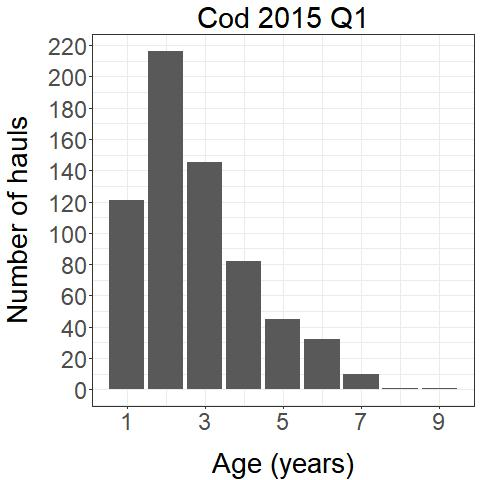
\includegraphics[width=0.28\textwidth]{figures/HaulsAndAgeHistograms/HaulsAndAge2015Q1Cod.jpeg}}
\qquad  
\subfloat[]{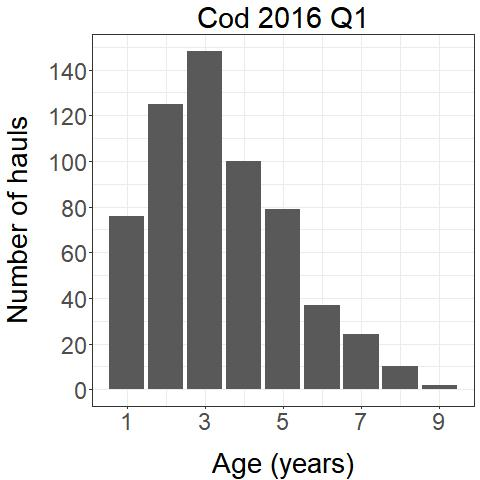
\includegraphics[width=0.28\textwidth]{figures/HaulsAndAgeHistograms/HaulsAndAge2016Q1Cod.jpeg}} \\
\qquad
\subfloat[]{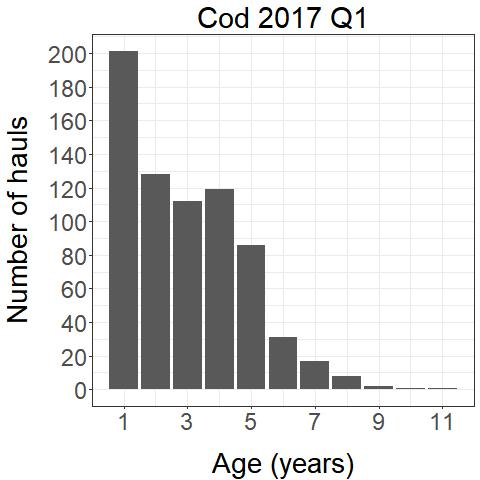
\includegraphics[width=0.28\textwidth]{figures/HaulsAndAgeHistograms/HaulsAndAge2017Q1Cod.jpeg}} 
\qquad
\subfloat[]{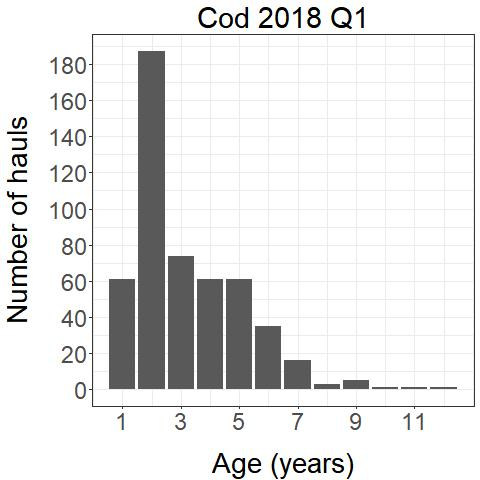
\includegraphics[width=0.28\textwidth]{figures/HaulsAndAgeHistograms/HaulsAndAge2018Q1Cod.jpeg}} \\
\qquad 
\subfloat[ ]{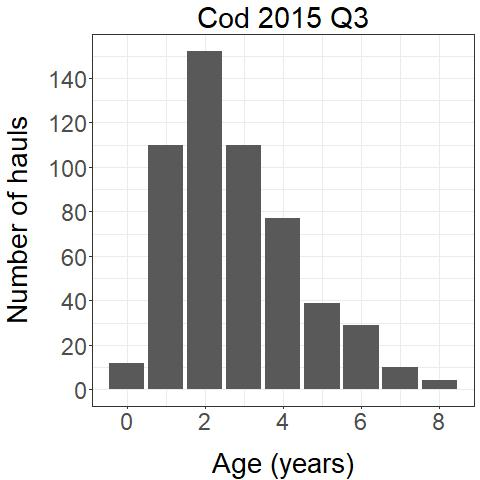
\includegraphics[width=0.28\textwidth]{figures/HaulsAndAgeHistograms/HaulsAndAge2015Q3Cod.jpeg}} 
\qquad
\subfloat[ ]{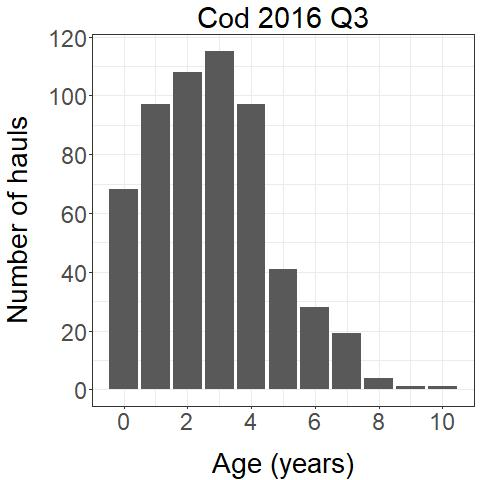
\includegraphics[width=0.28\textwidth]{figures/HaulsAndAgeHistograms/HaulsAndAge2016Q3Cod.jpeg}} \\
\qquad
\subfloat[ ]{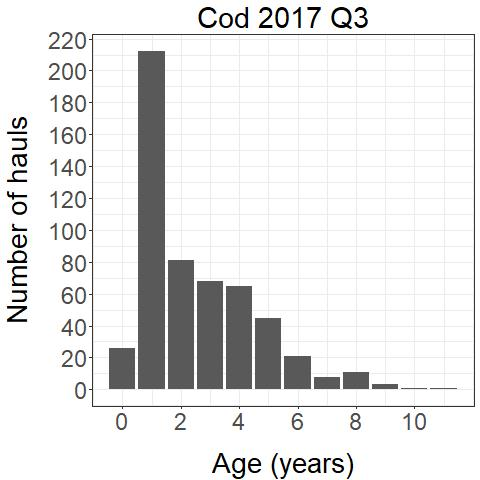
\includegraphics[width=0.28\textwidth]{figures/HaulsAndAgeHistograms/HaulsAndAge2017Q3Cod.jpeg}}
\qquad
\subfloat[ ]{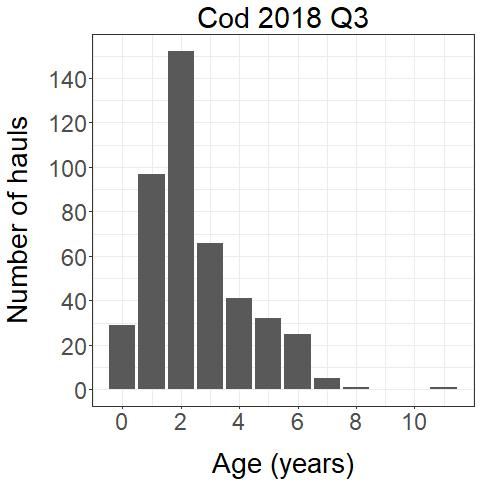
\includegraphics[width=0.28\textwidth]{figures/HaulsAndAgeHistograms/HaulsAndAge2018Q3Cod.jpeg}} 
\end{tabular}
\end{figure*} 



\clearpage
\begin{figure*}[h!]
\centering
\captionsetup{font=small, width = 14.5cm}{
\caption[]{The number of age 1 and 2-year old Cod sampled in hauls in 2015, 2016 and 2018.   }\label{AgeSCodALLYearsQ1}}
\begin{tabular}{@{}ccc@{}}
\subfloat[]{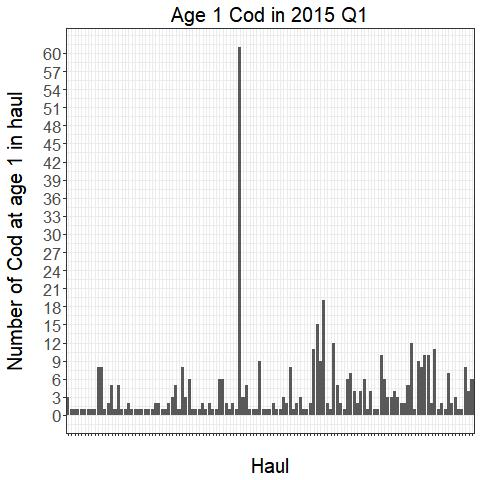
\includegraphics[width=0.4\textwidth]{figures/HaulsAndAgeHistograms/Age1Cod2015Q1.jpeg}}
\qquad
\subfloat[]{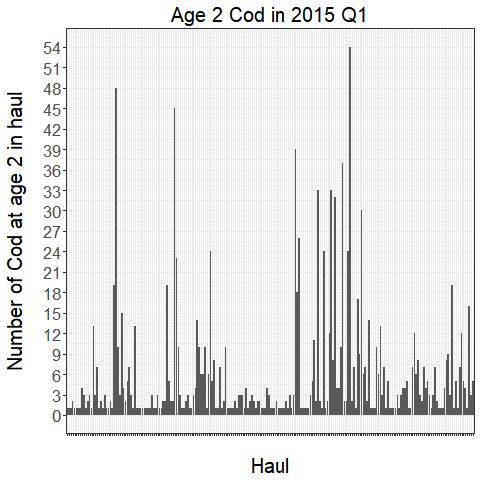
\includegraphics[width=0.4\textwidth]{figures/HaulsAndAgeHistograms/Age2Cod2015Q1.jpeg}} \\
\qquad 
\subfloat[]{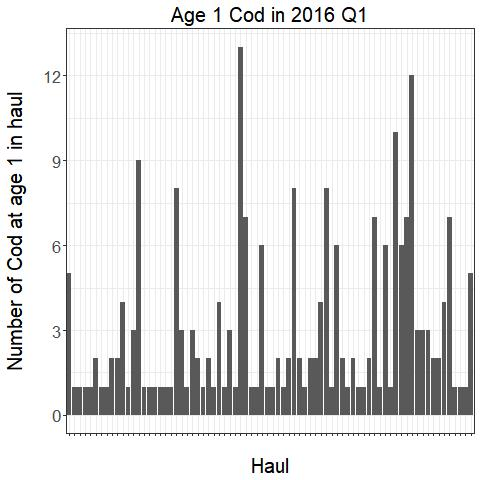
\includegraphics[width=0.4\textwidth]{figures/HaulsAndAgeHistograms/Age1Cod2016Q1.jpeg}}  
\qquad
\subfloat[]{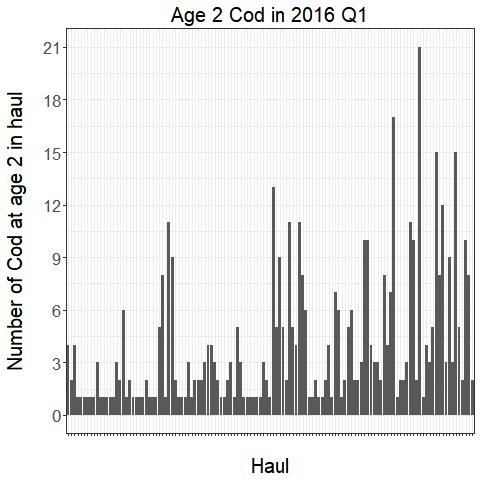
\includegraphics[width=0.4\textwidth]{figures/HaulsAndAgeHistograms/Age2Cod2016Q1.jpeg}}  \\
\qquad
\subfloat[]{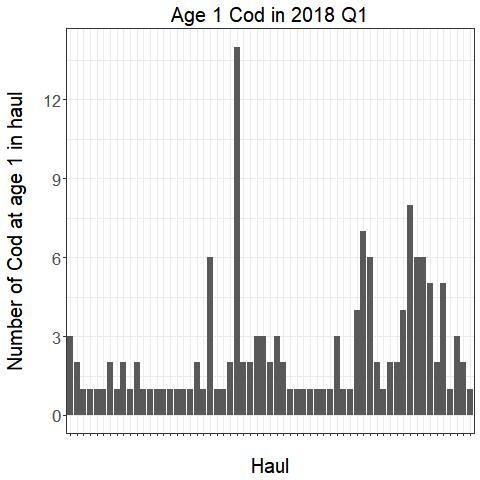
\includegraphics[width=0.4\textwidth]{figures/HaulsAndAgeHistograms/Age1Cod2018Q1.jpeg}}  
\qquad
\subfloat[]{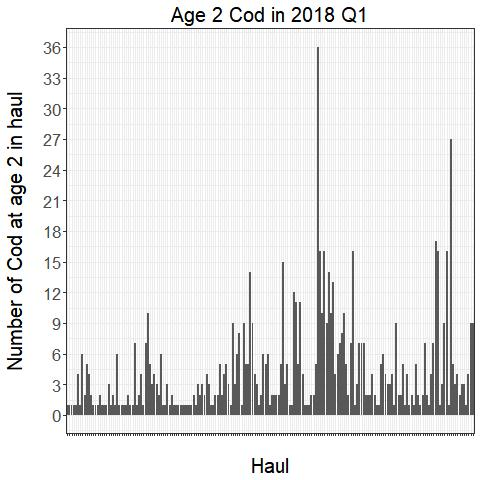
\includegraphics[width=0.4\textwidth]{figures/HaulsAndAgeHistograms/Age2Cod2018Q1.jpeg}}  
\end{tabular}
\end{figure*} 

%
% \clearpage
%
%\begin{figure*}[h!]
%\centering
%\begin{tabular}{@{}ccc@{}}
%\subfloat[ ]{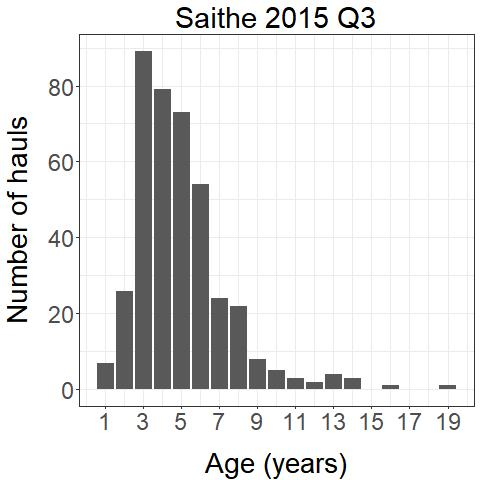
\includegraphics[width=0.28\textwidth]{figures/HaulsAndAgeHistograms/HaulsAndAge2015Q1Saithe.jpeg}} 
%\qquad
%\subfloat[ ]{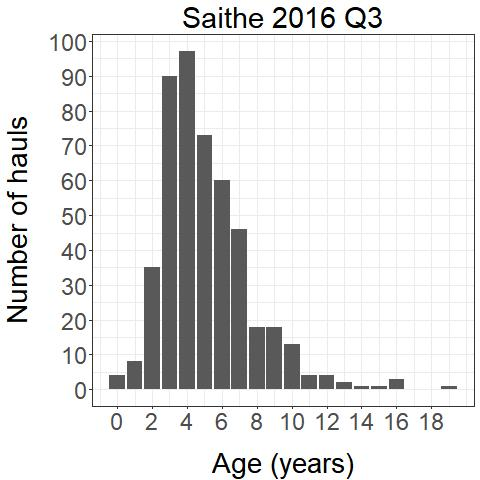
\includegraphics[width=0.28\textwidth]{figures/HaulsAndAgeHistograms/HaulsAndAge2016Q1Saithe.jpeg}} \\
%\qquad
%\subfloat[ ]{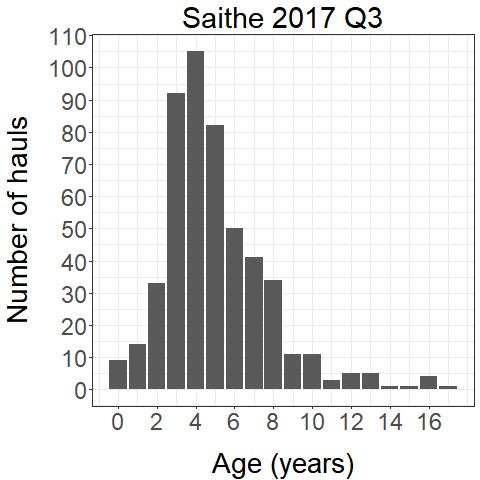
\includegraphics[width=0.28\textwidth]{figures/HaulsAndAgeHistograms/HaulsAndAge2017Q1Saithe.jpeg}}
%\qquad
%\subfloat[ ]{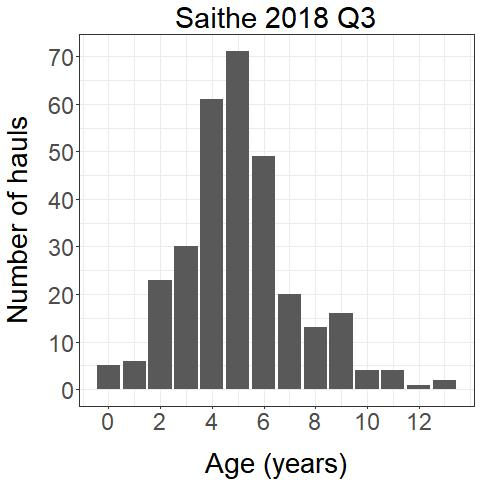
\includegraphics[width=0.28\textwidth]{figures/HaulsAndAgeHistograms/HaulsAndAge2018Q1Saithe.jpeg}} 
%\end{tabular}
%\captionsetup{font=small, width = 14.5cm}{
%\caption[]{Number of hauls with age data for North Sea  Saithe in quarter 3, respectively in the years 2015-2018. In Q3 surveys data is collected for age 0 group in the North Sea, however, no age 0 group data for Saithe were collected  in 2015 Q3.}
%\label{HaulsAgeTotalAllYearsSaithe}}
%\end{figure*} 
%
%
%\clearpage
%
%\begin{figure*}[h!]
%\centering
%\begin{tabular}{@{}ccc@{}}
%\subfloat[]{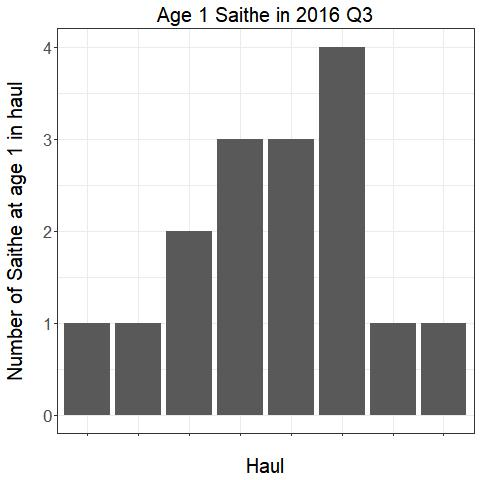
\includegraphics[width=0.4\textwidth]{figures/HaulsAndAgeHistograms/Age1Saithe2016Q3.jpeg}} 
%\qquad
%\subfloat[]{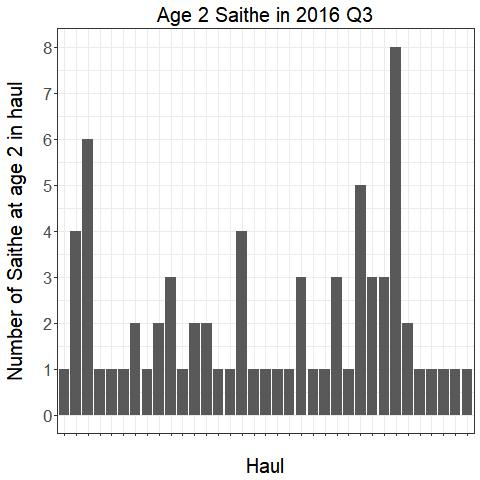
\includegraphics[width=0.4\textwidth]{figures/HaulsAndAgeHistograms/Age2Saithe2016Q3.jpeg}} \\
%\qquad 
%\subfloat[]{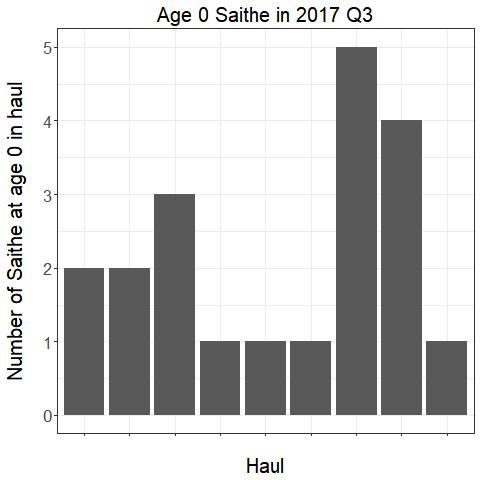
\includegraphics[width=0.4\textwidth]{figures/HaulsAndAgeHistograms/Age0Saithe2017Q3.jpeg}}  
%\qquad 
%\subfloat[]{\includegraphics[width=0.4\textwidth]{figures/HaulsAndAgeHistograms/Age1Saithe2017Q3.jpeg}}  \\
%\qquad
%\subfloat[]{\includegraphics[width=0.4\textwidth]{figures/HaulsAndAgeHistograms/Age1Saithe2018Q3.jpeg}}  
%\qquad 
%\subfloat[]{\includegraphics[width=0.4\textwidth]{figures/HaulsAndAgeHistograms/Age2Saithe2018Q3.jpeg}}  
%\end{tabular}
%\captionsetup{font=small, width = 14.5cm}{
%\caption[]{The number of age 0, 1 and 2-year old Saithe sampled in hauls in 2016-2018.  }\label{AgeSaitheALLYearsQ3}}
%\end{figure*} 
%



%%
%%\clearpage
% \begin{small}
%\begin{table}[h!]
%\setlength\tabcolsep{3.5pt} 
%\centering
%\captionsetup{font=small, width = 15cm}{
%\caption{Summary of North Sea Cod and Saithe data in years 2015-2018.  Data collected in the third quarter (Q3) has age 0 group but this is not collected in quarter 1 (Q1) surveys.}\label{tab:realdata2015-2018}}
%\begin{footnotesize}
%\begin{tabular}{clclclclclclclclclclclclclclclclclclclclclclclclclclclclclclclclclcl}
%  \hline \\ [0.3ex]
%{\bf Species} &  & \multicolumn{8}{c}{\bf Years and quarters} &   \\[1.0ex]
%%\hline\\
%%  \cmidrule(lr{0.3em}){3-6} \\ [0.5ex]% \cmidrule(lr{0.3em}){5-6}  \\ [0.5ex]
%&  & \multicolumn{2}{c}{2015} & \multicolumn{2}{c}{2016}  & \multicolumn{2}{c}{2017} & \multicolumn{2}{c}{2018}   \\ [1.0ex]
% \hline \\ [0.3ex]
%& & Q1  & Q3 & Q1  & Q3 & Q1  & Q3 & Q1  & Q3 & \\
%%\hline \\ 
%  \cmidrule(lr{0.3em}){3-10}  \\ [0.5ex]% \cmidrule(lr{0.3em}){13-20}  \\ [0.5ex]
% 	& Number of hauls   & 380 & 352 & 360 & 381 &377 & 337 & 372 &349   \\ [1.0ex]
% 	& Mean time of hauls (in minutes) & 28.55 & 23.44 & 28.40 & 22.47 &29.02 & 29.37 &  29.26 & 29.13 \\ [1.2ex]
%\raisebox{2.5ex}{\bf Cod}        \\ %   & Trawls &   &  &   & & &               & & 345 & 372 &   \\ [1.5ex]
%& Age range (in years)               & 1 - 9 & 0 - 8 & 1 - 10 & 0 - 10 & 1 - 11 & 0 - 11  &  1 - 12 & 0 - 11\\ [1.2ex]
%%& Length range (in cm)               & 9 - 113 &7 - 111 &11 - 109 & 5 - 110 & 7 - 115 & 6 - 112 &  11 - 114 & 5 - 107  \\[1.5ex] 
%& Total otoliths sampled for age determination               & 2895 &2113 & 2046 & 1804    &2501 & 2230  & 1600 & 1456 \\[1.2ex] 
%& Number of hauls with length data & 305 &216 & 251 & 230& 306 & 237  & 237 & 199 \\[1.2ex]
%& Number of hauls with age data    & 301 &209 & 243 & 224 & 293 & 236 & 229 & 195 \\[1.2ex]
%& Cod with missing age in RFAs     & 0.30\%& 0.13\% & 0.13\% & 0.34\% & 0.68\% &  0.07\% & 0.51\%  & 0.11\%  \\[1.2ex]  
%& Cod with missing age in hauls    & 10.06\% & 14.20\% & 6.18\%& 6.32\% & 2.25\% &0.27\%   & 1.40\%   & 0.77\% \\[2.2ex] 
%
%
%\raisebox{2.5ex}{\bf Saithe}        \\
%& Age range (in years)                         &1 - 16   & 0 - 19 &1 - 17   &0 - 19 &1 - 15 & 0 - 11 &  1 - 12 & 0 - 13 \\ [1.2ex]
%& Total otoliths sampled for age determination & 600  & 1526 & 581  &1631 &1083 & 2163  & 822 & 1085\\[1.2ex] 
%%& Length range (in cm)           & 13 - 110  & 21 - 109 & 16 - 107  & 12 - 115  &15 - 108 & 6 - 112 &  11 - 114 & 7 - 109     &  \\[1.5ex] 
%& Number of hauls with length data & 73 &117 &97 & 135& 122& 128  & 83 & 98\\[1.2ex]
%& Number of hauls with age data    & 71 &116 & 74& 132 & 111& 127 & 81 & 97\\[1.2ex]
%& Saithe with missing age in RFAs      &1.2\% & 0\%		& 0\%  & 0.03\% &0.14\%  &  0.05\% & 0.03\%  & 0\%  \\[1.2ex]  
%& Saithe with missing age in hauls     &21.6\%& 0.17\%	& 0.4\%&0.22\%  &20.1\%  &   0.08\% & 0.06\%  & 0.02\%  \\[0.5ex]
%
%   \hline \\[0.1ex]
%\end{tabular}
%\end{footnotesize}
%\end{table}
% \end{small}
% 

 
 
\clearpage


 \section{Real data analysis}
\label{secAP:realdataanalysis}

\subsection{Application of methods to North Sea Cod data in Q3 in years 2015-2018}
\label{secAp:applicationToCodData}

\subsubsection{Estimates from ALK estimators}
\label{secAp:estimatesFromALK}

In this section wee present the results from the two ALK methods for North Sea Cod in years 2015-2018 Q3. Figure \ref{HaulsAgeTotalAllYearsCod2018Q3} shows high variability between hauls. Catch rates of 3 and 4-year old North Cod are dominated in a single haul.

Figure \ref{AreaHaulEstimatesAllYearsQ3} gives the estimated point estimates and approximate 95\% confidence interval of the  mean catch per unit effort of North Sea Cod in years 2015-2018 Q3. The expected relative standard error (RSE) computed from the three bootstrap procedures (ICES, modified-ICES and stratified) are also given. The ALK methods gave similar point estimates of relative abundance and estimates of the variance because the variability in the ALK is considered in the estimation process. Higher RSEs are estimated for 4-year old north Sea Cod in 2018 Q3 because the variability is driven by a single haul (see Figure \ref{HaulsAgeTotalAllYearsCod2018Q3} 8 (b)).   \\


\begin{figure*}[h!]
\centering
\captionsetup{font=small, width = 14.5cm}{
\caption[]{Hauls containing 3 year-old and 4 year-old North Sea Cod in 2018 Q3. }\label{HaulsAgeTotalAllYearsCod2018Q3}}
\begin{tabular}{@{}ccc@{}}
\subfloat[]{\includegraphics[width=0.34\textwidth]{figures/HaulsAndAgeHistograms/Age3Cod2018Q3.jpeg}}
\qquad  
\subfloat[]{\includegraphics[width=0.34\textwidth]{figures/HaulsAndAgeHistograms/Age4Cod2018Q3.jpeg}}  
\end{tabular}
\end{figure*} 


\begin{figure*}[h!]
\centering
\captionsetup{font=small, width = 14.5cm}{
\caption[]{Estimated abundance-at-age for North Sea Cod for the two ALK estimators based on data from the International Bottom Trawl Survey in 2015-2018 in the third quarters Q3 (left panel). The error bars are estimated 95\% confidence intervals using the bias corrected (see Methods) and 500 bootstrap samples. Expected relative standard error (RSE) for estimated abundance-at-age (mCPUE) are also given in the right panel. The ICES-IBTS bootstrap procedure is compared with the modified ICES-IBTS and stratified bootstrap procedures. The ICES-IBTS bootstrap procedures are applied to the area based age-length key (ALK) and the stratified bootstrap procedure is applied to the haul based ALK. }\label{AreaHaulEstimatesAllYearsQ3}}
\begin{tabular}{@{}ccc@{}}
\subfloat[]{\includegraphics[width=0.33\textwidth]{figures/ALKplots/CodAreaHaulEstimates2015Q3.jpeg}} & 
\subfloat[]{\includegraphics[width=0.33\textwidth]{figures/BootstrapMethodsPlots/CodAreaHaulAreaMod2015Q3.jpeg}} & \\
\subfloat[]{\includegraphics[width=0.33\textwidth]{figures/ALKplots/CodAreaHaulEstimates2016Q3.jpeg}} & 
\subfloat[]{\includegraphics[width=0.33\textwidth]{figures/BootstrapMethodsPlots/CodAreaHaulAreaMod2016Q3.jpeg}} & \\
\subfloat[]{\includegraphics[width=0.33\textwidth]{figures/ALKplots/CodAreaHaulEstimates2017Q3.jpeg}} & 
\subfloat[]{\includegraphics[width=0.33\textwidth]{figures/BootstrapMethodsPlots/CodAreaHaulAreaMod2017Q3.jpeg}} & \\
\subfloat[]{\includegraphics[width=0.33\textwidth]{figures/ALKplots/CodAreaHaulEstimates2018Q3.jpeg}} & 
\subfloat[]{\includegraphics[width=0.33\textwidth]{figures/BootstrapMethodsPlots/CodAreaHaulAreaMod2018Q3.jpeg}} & 
\end{tabular}
\end{figure*} 

\clearpage

\subsubsection{Evaluating sampling strategies of age samples}
\label{secAp:evalutionofotoliths}

In this section we give the results for North Sea Cod in years 2015-2018 Q3. Table \ref{resamplingOtoliths2015-2018Q3} gives the average number of fish sampled to evaluate relative abundance-at-age for the various sampling strategies. The results suggest that the current number of fish sampled for age determination could be reduced by 45\% to give the same information concerning relative abundance-at-age. 

Figure \ref{fig:removalCodQ3} gives the expected RSE for the mean catch per unit effort at age of North Sea Cod in Q3 in years 2015-2018. The results show that the difference in expected RSE is minimal if \textit{one} fish is sampled in 1cm or 5cm length group width. Figure \ref{fig:removalCod5cmQ3} confirms that \textit{one} fish per 5cm length group width is sufficient for age determination of North Sea Cod.\\




\begin{small}
\begin{table}[h!]
\setlength\tabcolsep{6.5pt} 
\centering
\captionsetup{font=small, width = 15.5cm}{
\caption{Average number of fish sampled from 500 bootstrap replicates in length group widths: 5cm, 4cm, 3cm, 2cm, or 1cm (percentages are in parentheses). In each bootstrap replicate \textit{one} fish is sampled for age determination in each length group width in the third quarter in 2015-2018. Also, \textit{one}, \textit{two},  \textit{three},  \textit{four},  or \textit{five} fish are sampled in a 5cm length group width and the average number is given.  The total number of fish sampled in a given year of interest in IBTS is also given.}\label{resamplingOtoliths2015-2018Q3}}
\begin{footnotesize}
\begin{tabular}{clclclclclclclclclclclclclclclclclclclclclclclclclclclclclclclclclcl}
  \hline \\ [0.3ex]
{\bf Year} &   \multicolumn{5}{c}{\bf Length group width  } & \thead{\bf Total otoliths \\ \bf sampled in year of interest }  \\[1.0ex]
  & {5cm} & {4cm}  & {3cm} & {2cm}  & {1cm} \\ [1.0ex]
 \hline \\ [0.1ex]
	
{2015} &  926 (47\%) & 1023 (52\%)  & 1153 (58\%) & 1345 (68\%) & 1659 (84\%)  & 2113\\ [1ex]

{ 2016} & 964  (55\%) & 1034 (59\%)  & 1162 (66\%) & 1320 (76\%) & 1631 (94\%)  & 1804             & \\ [1ex]

{ 2017}   & 941  (41\%) & 1014 (44\%)  & 1172 (51\%) & 1394 (61\%) & 1795 (79\%)  & 2230             & \\ [1ex]

{ 2018} & 713  (49\%) & 790 (55\%)  & 865 (59\%) & 990 (68\%) & 1194 (82\%)  & 1456            & \\ [3ex]

& \multicolumn{5}{c}{\bf Number of fish sampled for age per 5cm length group width} \\[1.5ex]
& 1 & 2 & 3 & 4 & 5 \\
\cmidrule(lr{0.3em}){2-6} \\ [0.5ex]%
2015 & 926 (47\%) & 1364 (69\%)& 1609 (81\%)& 1747 (88\%)&1849 (93\%) & 2113 \\ [1ex]
2016 & 964 (55\%) & 1348 (77\%) & 208 (88\%)&1630 (93\%) & 1670 (96\%)& 1804\\ [1ex]
2017 &941 (41\%) & 1405 (61\%) & 1667 (73\%)& 1837 (81\%) & 1956 (86\%)& 2230  \\ [1ex]
2018 &713 (49\%) & 1012 (69\%)& 1170 (80\%) & 1255 (87\%)& 1303 (90\%) &  1456 \\ [1ex]


%\cmidrule(lr{0.3em}){2-6} \\ [0.5ex]%
%2015 &  (\%) & 1364 (69\%)& 1609 (81\%)& 1747 (88\%)&1849 (93\%) & 2113 \\ [1ex]
%2016 & (\%) & 1348 (77\%) & 208 (88\%)&1630 (93\%) & 1670 (96\%)& 1804\\ [1ex]
%2017 & (\%) & 1405 (61\%) & 1667 (73\%)& 1837 (81\%) & 1956 (86\%)& 2230  \\ [1ex]
%2018 & (\%) & 1012 (69\%)& 1170 (81\%) & 1255 (87\%)& 1303 (90\%) &  1456 \\ [1ex]
   \hline \\[0.1ex]
\end{tabular}
\end{footnotesize}
\end{table}
 \end{small}
 
 %The expected RSE with all the fish sampled for North Sea Cod is represented by the horizontal lines.
\clearpage
\begin{figure*}[h!]
\centering
\captionsetup{font=small, width = 14.5cm}{
\caption[]{Expected relative standard error of the mean catch per unit effort at age of North Sea Cod in Q3 in years 2015-2018 with different length group widths for 500 bootstrap samples. We sample \textit{one} fish in the following length group widths: 5cm, 4cm, 3cm, 2cm and 1cm, which is represented by the squares.  While the current sampling strategy recommended by ICES for North Sea Cod is \textit{one} fish sample per 1cm length group width, some nations sampled more than \textit{one} fish per 1cm. The numbers 1 through 6+ (and associated colours) represent the age of Cod, where 6+ is all fish of age 6 or older.}\label{fig:removalCodQ3}}
\begin{tabular}{@{}ccc@{}}
\subfloat[]{\includegraphics[width=0.4\textwidth]{results/olav/resamplingOtoliths/removalCod2015Q3.jpeg}} & 
\subfloat[]{\includegraphics[width=0.4\textwidth]{results/olav/resamplingOtoliths/removalCod2016Q3.jpeg}} & \\
\subfloat[]{\includegraphics[width=0.4\textwidth]{results/olav/resamplingOtoliths/removalCod2017Q3.jpeg}} & 
\subfloat[]{\includegraphics[width=0.4\textwidth]{results/olav/resamplingOtoliths/removalCod2018Q3.jpeg}} & 
\end{tabular}
\end{figure*} 

\clearpage
\begin{figure*}[h!]
\centering
\captionsetup{font=small, width = 14.5cm}{
\caption[]{Expected relative standard error of the mean catch per unit effort at age of North Sea Cod in Q3 in years 2015-2018 for varying number of fish sampled for age in a 5cm length group width: \textit{one}, \textit{two}, \textit{three}, \textit{four} or \textit{five} fish sampled for age is represented by the squares.  The expected RSE for all fish currently sampled per length group in the North Sea, denoted by ``c", is represented by the circle. The current sampling strategy recommended by ICES from 2018 Q1 for North Sea Cod is \textit{one} fish per 1cm length group width from each trawl haul, although some nations still sampled more than one fish for age determination per 1cm length group width.}\label{fig:removalCod5cmQ3}}
\begin{tabular}{@{}ccc@{}}
\subfloat[]{\includegraphics[width=0.36\textwidth]{results/olav/resamplingOtoliths/removalCod2015Q3DL5.jpeg}} & 
\subfloat[]{\includegraphics[width=0.36\textwidth]{results/olav/resamplingOtoliths/removalCod2016Q3DL5.jpeg}} & \\
\subfloat[]{\includegraphics[width=0.36\textwidth]{results/olav/resamplingOtoliths/removalCod2017Q3DL5.jpeg}} & 
\subfloat[]{\includegraphics[width=0.36\textwidth]{results/olav/resamplingOtoliths/removalCod2018Q3DL5.jpeg}} & 
\end{tabular}
\end{figure*} 

 \subsubsection{Evaluating sampling strategies of age samples and number of hauls in IBTS Q3 surveys}
\label{secAp:evalutionofotolithsAndHauls}
In this section we give the expected relative standard error (RSE) for  North Sea Cod in Q3 in years 2015-2018 when sampling \textit{one}  or \textit{five} fish in length group width 5cm for age determination. Estimates are provided for 500 bootstrap samples. The results show that there is no real difference in expected RSE for \textit{one} or \textit{five} fish sampled for age determination of North Sea Cod. But at least 300 hauls are required for the RSEs to approach their asymptotic limit.

\clearpage
\begin{figure*}[h!]
\centering
\captionsetup{font=small, width = 14.5cm}{
\caption[]{Expected relative standard error (RSE) for North Sea Cod in Q3 in years 2015-2016 when sampling \textit{one} (red line) or \textit{five} (black line) fish in length group width 5cm for 500 bootstrap samples. For each sampling strategy of otoliths, the area based ALK is used for the given number of hauls, $N= 50, 75, 100, 150, 200, 250, 300, 350, 400, 500$.   }\label{OtolithHauls2015-2016Q3}}
\begin{tabular}{@{}ccc@{}}
\subfloat[]{\includegraphics[width=0.93\textwidth]{results/olav/resamplingNandotoliths/resampleNandOcod2015Q3DL5datras.jpeg}} & \\
\subfloat[]{\includegraphics[width=0.93\textwidth]{results/olav/resamplingNandotoliths/resampleNandOcod2016Q3DL5datras.jpeg}} & 
\end{tabular}
\end{figure*} 


\clearpage

\begin{figure*}[h!]
\centering
\captionsetup{font=small, width = 14.5cm}{
\caption[]{Expected relative standard error (RSE) for Cod in Q3 in years 2017-2018 when sampling \textit{one} (red line) or \textit{five} (black line) pairs of otoliths in length group width 5cm for 500 bootstrap samples. For each sampling strategy of otoliths, the area based ALK is used for the given number of hauls, $N= 50, 75, 100, 150, 200, 250, 300, 350, 400, 500$.   }\label{OtolithHauls2017-2018Q3}}
\begin{tabular}{@{}ccc@{}}
\subfloat[]{\includegraphics[width=0.93\textwidth]{results/olav/resamplingNandotoliths/resampleNandOcod2017Q3DL5datras.jpeg}} & \\
\subfloat[]{\includegraphics[width=0.93\textwidth]{results/olav/resamplingNandotoliths/resampleNandOcod2018Q3DL5datras.jpeg}} & 
\end{tabular}
\end{figure*} 


\clearpage

\subsubsection{Evaluating sampling strategies of age samples and number of hauls in IBTS surveys in years 1997-1999}
\label{secAp:evalutionofotolithsAndHauls1997-1999}

In this section we present estimates of abundance-at-age of North Sea Cod in years 1997-1999 in the first and third quarters. We set the number of hauls to  $N= 50, 75, 100, 200, 300, 400, 500$ and investigate the espected relative standard error if \textit{one} or \textit{five} fish are sampled per 5cm length group width.\\

 
\begin{figure*}[h!]
\centering
\captionsetup{font=small, width = 14.5cm}{
\caption[]{Expected relative standard error (RSE) for North Sea Cod in Q1 in year 1997 when sampling \textit{one} (red line) or \textit{five} (black line) fish in length group width 5cm for 500 bootstrap samples. For each sampling strategy of otoliths, the area based ALK is used for the given number of hauls, $N= 50, 75, 100, 200, 300, 400, 500$.   }\label{OtolithHauls1997Q3}}
\begin{tabular}{@{}ccc@{}}
\subfloat[]{\includegraphics[width=1.05\textwidth]{results/olav/resamplingNandotoliths/resampleNandOcod1997Q1DL5datras.jpeg}} & \\
%\subfloat[]{\includegraphics[width=0.95\textwidth]{results/olav/resamplingNandotoliths/resampleNandOcod1998Q3DL5datras.jpeg}} & 
\end{tabular}
\end{figure*} 


\clearpage
\begin{figure*}[h!]
\centering
\captionsetup{font=small, width = 14.5cm}{
\caption[]{Expected relative standard error (RSE) for North Sea Cod in Q1 in year 1998 when sampling \textit{one} (red line) or \textit{five} (black line) fish in length group width 5cm for 500 bootstrap samples. For each sampling strategy of otoliths, the area based ALK is used for the given number of hauls, $N=  50, 75, 100, 200, 300, 400, 500$.   }\label{OtolithHauls1997Q3}}
\begin{tabular}{@{}ccc@{}}
\subfloat[]{\includegraphics[width=1.05\textwidth]{results/olav/resamplingNandotoliths/resampleNandOcod1998Q1DL5datras.jpeg}} & \\
%\subfloat[]{\includegraphics[width=0.95\textwidth]{results/olav/resamplingNandotoliths/resampleNandOcod1998Q3DL5datras.jpeg}} & 
\end{tabular}
\end{figure*} 


\clearpage
\begin{figure*}[h!]
\centering
\captionsetup{font=small, width = 14.5cm}{
\caption[]{Expected relative standard error (RSE) for Cod in Q1 in year 1999 when sampling \textit{one} (red line) or \textit{five} (black line) pairs of otoliths in length group width 5cm for 500 bootstrap samples. For each sampling strategy of otoliths, the area based ALK is used for the given number of hauls, $N= 50, 75, 100, 200, 300, 400, 500$.   }\label{OtolithHauls1999Q3}}
\begin{tabular}{@{}ccc@{}}
\subfloat[]{\includegraphics[width=1.05\textwidth]{results/olav/resamplingNandotoliths/resampleNandOcod1999Q1DL5datras.jpeg}} & \\
%\subfloat[]{\includegraphics[width=0.95\textwidth]{results/olav/resamplingNandotoliths/resampleNandOcod2018Q3DL5datras.jpeg}} & 
\end{tabular}
\end{figure*} 




\clearpage


\begin{figure*}[h!]
\centering
\captionsetup{font=small, width = 14.5cm}{
\caption[]{Expected relative standard error (RSE) for North Sea Cod in Q3 in year 1997 when sampling \textit{one} (red line) or \textit{five} (black line) fish in length group width 5cm for 500 bootstrap samples. For each sampling strategy of otoliths, the area based ALK is used for the given number of hauls, $N= 25, 50, 75, 100, 200, 300, 400, 500$.   }\label{OtolithHauls1997Q3}}
\begin{tabular}{@{}ccc@{}}
\subfloat[]{\includegraphics[width=1.05\textwidth]{results/olav/resamplingNandotoliths/resampleNandOcod1997Q3DL5datras.jpeg}} & \\
%\subfloat[]{\includegraphics[width=0.95\textwidth]{results/olav/resamplingNandotoliths/resampleNandOcod1998Q3DL5datras.jpeg}} & 
\end{tabular}
\end{figure*} 


\clearpage
\begin{figure*}[h!]
\centering
\captionsetup{font=small, width = 14.5cm}{
\caption[]{Expected relative standard error (RSE) for North Sea Cod in Q3 in year 1998 when sampling \textit{one} (red line) or \textit{five} (black line) fish in length group width 5cm for 500 bootstrap samples. For each sampling strategy of otoliths, the area based ALK is used for the given number of hauls, $N= 25, 50, 75, 100, 200, 300, 400, 500$.   }\label{OtolithHauls1997Q3}}
\begin{tabular}{@{}ccc@{}}
\subfloat[]{\includegraphics[width=1.05\textwidth]{results/olav/resamplingNandotoliths/resampleNandOcod1997Q3DL5datras.jpeg}} & \\
%\subfloat[]{\includegraphics[width=0.95\textwidth]{results/olav/resamplingNandotoliths/resampleNandOcod1998Q3DL5datras.jpeg}} & 
\end{tabular}
\end{figure*} 


\clearpage
\begin{figure*}[h!]
\centering
\captionsetup{font=small, width = 14.5cm}{
\caption[]{Expected relative standard error (RSE) for Cod in Q3 in year 1999 when sampling \textit{one} (red line) or \textit{five} (black line) pairs of otoliths in length group width 5cm for 500 bootstrap samples. For each sampling strategy of otoliths, the area based ALK is used for the given number of hauls, $N= 25,50, 75, 100, 200, 300, 400, 500$.   }\label{OtolithHauls1999Q3}}
\begin{tabular}{@{}ccc@{}}
\subfloat[]{\includegraphics[width=1.05\textwidth]{results/olav/resamplingNandotoliths/resampleNandOcod1999Q3DL5datras.jpeg}} & \\
%\subfloat[]{\includegraphics[width=0.95\textwidth]{results/olav/resamplingNandotoliths/resampleNandOcod2018Q3DL5datras.jpeg}} & 
\end{tabular}
\end{figure*} 


\end{document}